\section{Introducción}
\subsection{Maple Flow}
Maple Flow es una nueva herramienta de cálculo de Maplesoft. Maple Flow ofrece una interfaz de usuario de forma libre combinada con un motor matemático integral. Utilice Maple Flow para cálculos y documentación de ingeniería, científicos y técnicos.

\newp

Maple Flow te da:

\begin{itemize}
	\item Un lienzo matemático espacialmente consciente que replica la metáfora del diseño de una pizarra física
	
	\item Recálculo automático para garantizar que los resultados estén siempre actualizados
	
	\item Un lenguaje matemático amplio y rico con muchas funciones
	
	\item Tramas visualmente impactantes, completamente programáticas
	
	\item Una región de codificación con acceso completo al lenguaje de programación Maple
	
\end{itemize}

Nota para usuarios que no son de Windows: Las pulsaciones de teclas que se dan en este documento son para Windows. Si está utilizando una plataforma diferente, consulte los métodos abreviados de teclado para su plataforma en Métodos abreviados de teclado (página 34).

\subsection{¿Qué pretende hacer este manual?}
Este manual describe

\begin{itemize}
  \item La interfaz Maple Flow
  
  \item Diferencias con la interfaz de usuario de Maple y el lenguaje de programación que un usuario existente de Maple puede experimentar.

\end{itemize}

Este manual debe leerse al unísono con los tutoriales y ejercicios del producto; estos están disponibles en el enlace Tutorial en la página de inicio de Maple Flow. Si ha cerrado la página de inicio, puede volver a acceder a ella desde el menú Ver:

\begin{itemize}
  \item Seleccione Ver $>$ Inicio Tutorial		
\end{itemize}

\insertimage[]{2022_12_20_3e2ffe6ad124ec91ee5cg-08}{width=10cm}{Descripción general de los tutoriales del producto.}	

Este manual no describe la funcionalidad matemática de Maple Flow en detalle, pero hace referencia a funciones específicas en el contexto de una discusión más amplia. La documentación detallada de la funcionalidad matemática se encuentra en la ayuda en línea de Maple: \href{http://www.maplesoft.com/support/help}{http://www.maplesoft.com/support/help}.

\subsection{¿Cuál es la relación entre Maple y Maple Flow?}
Primero, algunas definiciones:

\begin{itemize}
	\item Maple se refiere al (i) lenguaje de programación Maple y (ii) la interfaz Maple.

	\item Maple Flow se refiere al nuevo producto cuyo manual está leyendo.
\end{itemize}

Maple Flow

\begin{itemize}
  \item Está construido sobre el lenguaje de programación Maple
  
  \item Toma prestados algunos elementos de la interfaz de Maple
\end{itemize}

El "lenguaje" de Maple Flow son los comandos (y su sintaxis), las estructuras de datos y el lenguaje de programación. Estos se basan en el lenguaje de programación Maple; puede utilizar cualquiera de las funciones matemáticas de Maple en sus análisis de Maple Flow.

Maple se instala automáticamente cuando instala Maple Flow.

\subsection{Si eres usuario de Maple}
Si ya usa Maple, apreciará el giro único que ofrece Maple Flow con su modelo de evaluación espacial y las actualizaciones automáticas de cálculo. También obtendrá una ventaja inicial porque estará familiarizado con el lenguaje de programación, las funciones y las características de Maple.

Maple Flow se diferencia de la interfaz y el lenguaje de programación de Maple en varios aspectos. Varias diferencias importantes se enumeran en la Tabla 1.1.

\insertimage[]{2022_12_20_3e2ffe6ad124ec91ee5cg-09}{width=\textwidth}{Tabla 1.1: En qué se diferencia Maple Flow de Maple.}

Las hojas de trabajo de Maple no se pueden cargar en Maple Flow, o viceversa.

\subsection{Sistema de ayuda Maple Flow}
El sistema de ayuda del producto, al que se accede a través del menú Ayuda, proporciona información sobre más de 130 comandos clave. Cada página de ayuda brinda detalles sobre el uso de un comando, incluida la secuencia de llamada, los parámetros, las opciones y los ejemplos.

Buscar: busque un nombre de comando, una palabra clave o una frase.

Examinar: explore la tabla de contenido para ver una lista estructurada de temas de ayuda

Ver página de ayuda como hoja de trabajo: puede abrir cualquier página de ayuda como hoja de trabajo para interactuar con la página y modificar los ejemplos.

\begin{itemize}
  \item Con la página de ayuda mostrada en el panel derecho del sistema de ayuda, desde el menú Ver, seleccione Abrir página como hoja de trabajo. Se abre una nueva ventana de hoja de cálculo. 
  \item Como alternativa, haga clic en Abrir la página actual como hoja de trabajo (ws) en la barra de herramientas del sistema de ayuda.
\end{itemize}

\textbf{Documentación adicional}
Dado que Maple Flow utiliza el lenguaje de programación Maple, tiene la capacidad de utilizar la amplia funcionalidad matemática que forma parte del lenguaje de programación Maple. Al navegar por el sistema de ayuda, algunos hipervínculos lo llevan a documentación detallada adicional para la funcionalidad matemática que reside en el sitio web de Maplesoft, en la ayuda en línea de Maple:

\href{http://www.maplesoft.com/support/help}{http://www.maplesoft.com/support/help}. Tenga en cuenta que estas páginas están formateadas como páginas de Maple, no como páginas de Maple Flow, por lo que los ejemplos se verán un poco diferentes.

\subsection{Interfaz}
Las diferentes partes de la interfaz Maple Flow, como se ve en la Figura 1.2, son:

\begin{itemize}
  \item Canvas - el espacio de trabajo

\item Barra de herramientas principal - Esta barra de herramientas siempre está en la parte superior de la ventana de Maple Flow.

\item Barra de herramientas contextual: esta barra de herramientas, ubicada directamente sobre el lienzo, es relevante para la selección actual.

\item Paletas : en el panel izquierdo, proporcionan una manera fácil de ingresar una expresión matemática, matriz, letra griega o unidades.

\item Panel de contexto: aquí aparecen algunas opciones relevantes para la selección actual, como formato numérico y formato de unidades.

\item Barra de estado — Muestra información del sistema
\end{itemize}
\insertimage[\label{img::1.2}]{ 2022_12_20_3e2ffe6ad124ec91ee5cg-10}{width=17cm}{La interfaz Maple Flow.}

\textbf{Personalizar la interfaz}
Personalice sus preferencias de Maple Flow utilizando el cuadro de diálogo Opciones.

Para abrir el cuadro de diálogo Opciones:

\begin{itemize}
  \item En la barra de herramientas, haga clic en el icono Opciones ( $\boldsymbol{*})$. Hay dos pestañas. En la pestaña Mostrar, puede especificar el número predeterminado de lugares decimales para usar al redondear los resultados. Para obtener más información, consulte Formato numérico (página 10).
\end{itemize}

En la pestaña Interfaz, puede especificar lo siguiente:

\begin{itemize}
  \item Abrir hojas de trabajo en una nueva pestaña o nueva ventana.

\item Abrir hipervínculos en una nueva pestaña o nueva ventana.

\item Zoom predeterminado.
\end{itemize}

Haga clic en Aplicar a la sesión para aplicar solo para la sesión actual de Maple Flow, o haga clic en Aplicar globalmente para aplicar la configuración a la sesión actual y a sesiones futuras.

\insertimage[\label{img::2.2}]{2022_12_20_3e2ffe6ad124ec91ee5cg-11}{width=10cm}{Diálogo de opciones.}

\section{Canvas}
\subsection{Grid}
Cuando arrastra contenedores matemáticos y de texto, las posiciones de los contenedores se ajustan a una cuadrícula. De forma predeterminada, la cuadrícula no se muestra.

Para mostrar la cuadrícula, haga clic en el botón Habilitar/Deshabilitar cuadrícula en la barra de herramientas principal.

\insertimage[\label{img::2.1}]{2022_12_20_3e2ffe6ad124ec91ee5cg-12}{width=10cm}{botón Activar/Desactivar cuadrícula en la barra de herramientas.}

\subsection{Cursor de cuadrícula}
El cursor de cuadrícula se ilustra en la Figura $\mathbf{2. 2}$ y por defecto aparece en la esquina superior izquierda de cada lienzo nuevo.

%Cursor de cuadrícula
El cursor de la cuadrícula se puede mover apuntando y haciendo clic con el mouse o con las teclas de flecha.

Los contenedores matemáticos y de texto se crean en la ubicación del cursor de cuadrícula.

\subsection{Contenedores de texto y matemáticas}
En el lienzo, puede crear cuadros matemáticos o cuadros de texto. Cada caja se puede mover; la posición de un contenedor matemático determina el orden en que se evalúa (como se ilustra en la Figura 3.9).

Un contenedor puede estar en uno de tres estados, como se describe en la Tabla 2.1.
\insertimage[\label{img::2.1}]{2022_12_20_3e2ffe6ad124ec91ee5cg-12(1)}{width=17cm}{Tabla 2.1: Estados del contenedor.}



\begin{center}
\begin{tabular}{|l|l|l|}
\hline
 & Math & Text \\
\hline
- One or several containers can be in move &  &  \\
mode. &  &  \\
- Move the containers with the mouse. &  &  \\
- When instead you select using the &  &  \\
keyboard and Ctrl key, the container has &  &  \\
a royal blue border. &  &  \\
- Move the container with Ctrl + arrow &  &  \\
keys. &  & $\mathrm{x}^{2}=9$ \\
\hline
\end{tabular}
\end{center}

\subsection{Moving Containers}
\section{Single Container}
With the mouse

To move a container with the mouse:

\begin{enumerate}
  \item Move the mouse pointer over a container.

  \item Move the container to another position by click and dragging.

  \item Release the mouse button when the container is in the desired position.

\end{enumerate}

\section{With the keyboard arrows}
To move a container with the keyboard:

\begin{enumerate}
  \item Move the grid cursor into a container so that the container is in editing mode.

  \item Do one of the following:

\end{enumerate}

\begin{itemize}
  \item Press Ctrl and use the arrow keys to move the container one grid space at a time.

  \item Press Ctrl + Shift and use the arrow keys to move the container a single pixel at a time.

\end{itemize}

Note that when you press Ctrl, the container border changes to royal blue to indicate $\mathbf{C t r l}$ has been pressed.

\section{Group of Containers}
To move multiple containers:

\begin{enumerate}
  \item Click in a blank part of the canvas.

  \item Drag a selection box around a group of containers.

  \item Release the mouse button.

  \item Move the mouse pointer over one of the selected containers.

  \item Drag the containers to another location.

\end{enumerate}

\section{Bringing Containers from Back to Front, and Vice Versa}
You can potentially have two containers at the same grid position.You can bring the lower container forward, or send the top container back, by using Flip to Front and Flip to Back buttons.

\begin{center}

\includegraphics[max width=\textwidth]{2022_12_20_3e2ffe6ad124ec91ee5cg-13}
\end{center}

Figure 2.3: Flip to Front and Flip to Back buttons

\subsection{Editing an Existing Container}
To enter editing mode on an existing container, do one of the following:

\begin{itemize}
  \item With the mouse, click the container.

  \item With the arrow keys, move the grid cursor onto the container.

\end{itemize}

\subsection{Deleting a Container}
To remove a container, do one of the following:

\begin{itemize}
  \item With the mouse, select the container (or containers) and from the toolbar, select Cut (O)

  \item Move the grid cursor into a container so that the container is in editing mode. Then press Ctrl + Delete to delete the in-focus container.

\end{itemize}

\subsection{Inserting or Removing White Space}
You can insert or remove space in the canvas (i.e. grid rows) by using the Enter, Backspace, and Delete keys.

\section{Adding Blank Rows}
To add blank rows, place the grid cursor on a blank part of the canvas and press Enter. This shifts all content on and below the same row as the grid cursor down.

\section{Deleting Blank Rows}
To delete blank rows, click on a blank row of the canvas and press one of the following:

\begin{itemize}
  \item Backspace to remove that blank row and shift the grid cursor and all content below the grid cursor up

  \item Delete to remove that blank row, and shift all content below that row up.

\end{itemize}

\section{Entering Math}
\subsection{Creating a Math Container}
A math container is a box in which you enter math that is to be evaluated.

To create a math container:

\begin{enumerate}
  \item Click on a blank part of the canvas.

  \item Begin typing your math. As soon as you enter the first character, a math container is created automatically.

\end{enumerate}

\subsection{Deleting a Math Container}
To delete a math container, do one of the following:

\begin{itemize}
  \item Drag-select the math container and press Delete.

  \item In editing mode, press Ctrl + Delete to delete the in-focus container.

\end{itemize}

\subsection{Evaluating Math and Displaying Output}
All math is evaluated in the canvas, using a left-to-right, top-to-bottom order (see Evaluation Order (page 14)). When you need to display results, evaluate and display output.

To evaluate math and display output:

\begin{enumerate}
  \item Enter the expression, then with the cursor at the right end of the expression, press $=$.

  \item Press Enter or the arrow keys. The result is displayed. After evaluation, the focus leaves the math container.

\end{enumerate}

\subsection{Numeric and Symbolic Evaluation Modes}
Maple Flow offers two math evaluation modes - numeric and symbolic.

Table 3.1: Difference between numeric and symbolic evaluation modes

\begin{center}
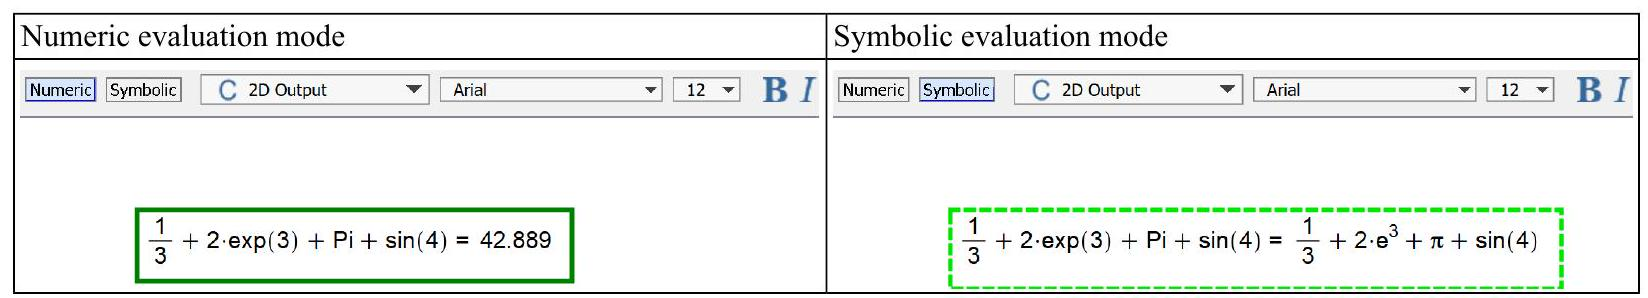
\includegraphics[max width=\textwidth]{2022_12_20_3e2ffe6ad124ec91ee5cg-15}
\end{center}

The numeric evaluation mode performs as much numeric evaluation as possible. For example:

\begin{itemize}
  \item Rational fractions (such as $1 / 2$ ) are converted to floating-point numbers

  \item Pi and $\exp (1)$ evaluate to floating-point numbers

\end{itemize}

Symbolic evaluation mode prevents numeric evaluation (except when requested by the user). For example:

\begin{itemize}
  \item Rational fractions are only converted to floating-point numbers if request by the user (e.g. with the evalf command)

  \item Pi evaluates to a symbolic name

\end{itemize}

In both modes, unassigned names are evaluated symbolically (i.e. in numeric mode, unassigned names do not give an error when evaluated).

The current mode of an existing math container is given by clicking inside it, and observing the state of the border or Numeric/Symbolic buttons in the Context toolbar, as illustrated in Table 3.1. By default, new math containers are numeric. Clicking the Symbolic button in the Context toolbar switches the in-focus math container to symbolic mode. Alternatively, use the shortcut key Alt $+\mathbf{S}$.

Holding down the Symbolic button for a second makes symbolic evaluation mode "sticky". This is indicated with a padlock by the Symbolic button ( 5 Symbolic ${ }^{A}$ ). This means that all future math containers will be symbolic (until symbolic mode is toggled off, by toggling to Numeric, or with another long click on the Symbolic button).

\subsection{Numeric Formatting}
By default, Maple Flow displays numeric results with three decimal places. To customize the numeric formatting:

\begin{enumerate}
  \item Place the editing cursor on a numeric result.

  \item Use the Number Format options in the Context Panel.

\end{enumerate}

\begin{center}
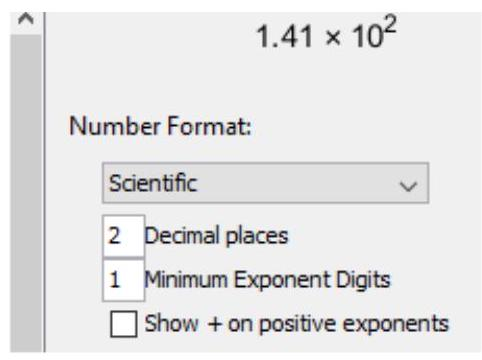
\includegraphics[max width=\textwidth]{2022_12_20_3e2ffe6ad124ec91ee5cg-16}
\end{center}

Figure 3.1: Numeric formatting

Note that the number format options in the Context Panel only apply to a single math container.

To select a number format and apply it broadly, you can use the Options Dialog to set your desired number format and apply it either to the current session or globally.

\begin{enumerate}
  \item From the toolbar, click the Options icon ( 4 ).

  \item Under the Display tab, select the desired number format.

  \item Click Apply to Session to apply for the current Maple Flow session only, or click Apply Globally to apply the setting to the current session and future sessions.

\end{enumerate}

\begin{center}
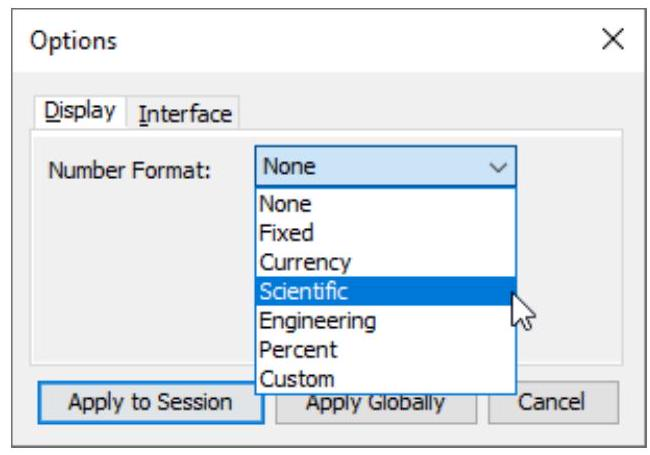
\includegraphics[max width=\textwidth]{2022_12_20_3e2ffe6ad124ec91ee5cg-16(1)}
\end{center}

Figure 3.2: Setting default numeric formatting

Maple Flow supports the following standard number formats:

\begin{itemize}
  \item Fixed

  \item Currency

  \item Scientific - Engineering

  \item Percent

\end{itemize}

You can also create a Custom format.

To apply a custom format to a single math container:

\begin{enumerate}
  \item Place the cursor in the numeric result to be formatted.

  \item In the Context Panel, under Number Format, select Custom. In the custom string field you can enter a string that is specific to your formatting needs.

\end{enumerate}

Examples include the following:

\begin{itemize}
  \item \#.\#\#\# formats to $3.12$

  \item $00.000$ formats to $03.120$

  \item \#,\#.\# formats to $2,100,320.5$

  \item $\$ 0.00$ formats to $\$ 123.50$

  \item ??0.00;\href{??0.00}{Red} formats to blue for a positive number, and red for a negative number

  \item $[<10]$ Low; [>=100]High;Medium formats to "Low" for numbers less than 10,"High" for numbers less than or equal to 100, and "Medium" otherwise

\end{itemize}

\section{To apply a custom format to all numeric results in the current session or globally:}
\begin{enumerate}
  \item From the toolbar, click the Options icon ( $\nLeftarrow$ ).

  \item Under the Display tab, for Number Format select Custom and enter your specification in the custom string field.

  \item Click Apply to Session to apply for the current Maple Flow session only, or click Apply Globally to apply the setting to the current session an future sessions.

\end{enumerate}

To remove a number format, return to the Number Format dialog and select None.

\subsection{Creating a Definition}
You can assign a numerical value or an expression to a name by using := (a colon, followed by an equal sign).

For example, entering a:=4 in a math container assigns the value 4 to the name a.

\subsection{Basic Arithmetic}
Equations are entered in typeset math notation, using standard keys such as $/, *,+$ and $-$.

Note that multiplication must always be explicitly stated. For example, you must enter $3 * \mathrm{x}$, not $3 \mathrm{x}$.

You can also use the Expression palette or Command Completion feature to enter typeset math, as illustrated in Table 3.2. Table 3.2: Using the Command Completion feature and Expression Palette to insert a square root

\begin{center}
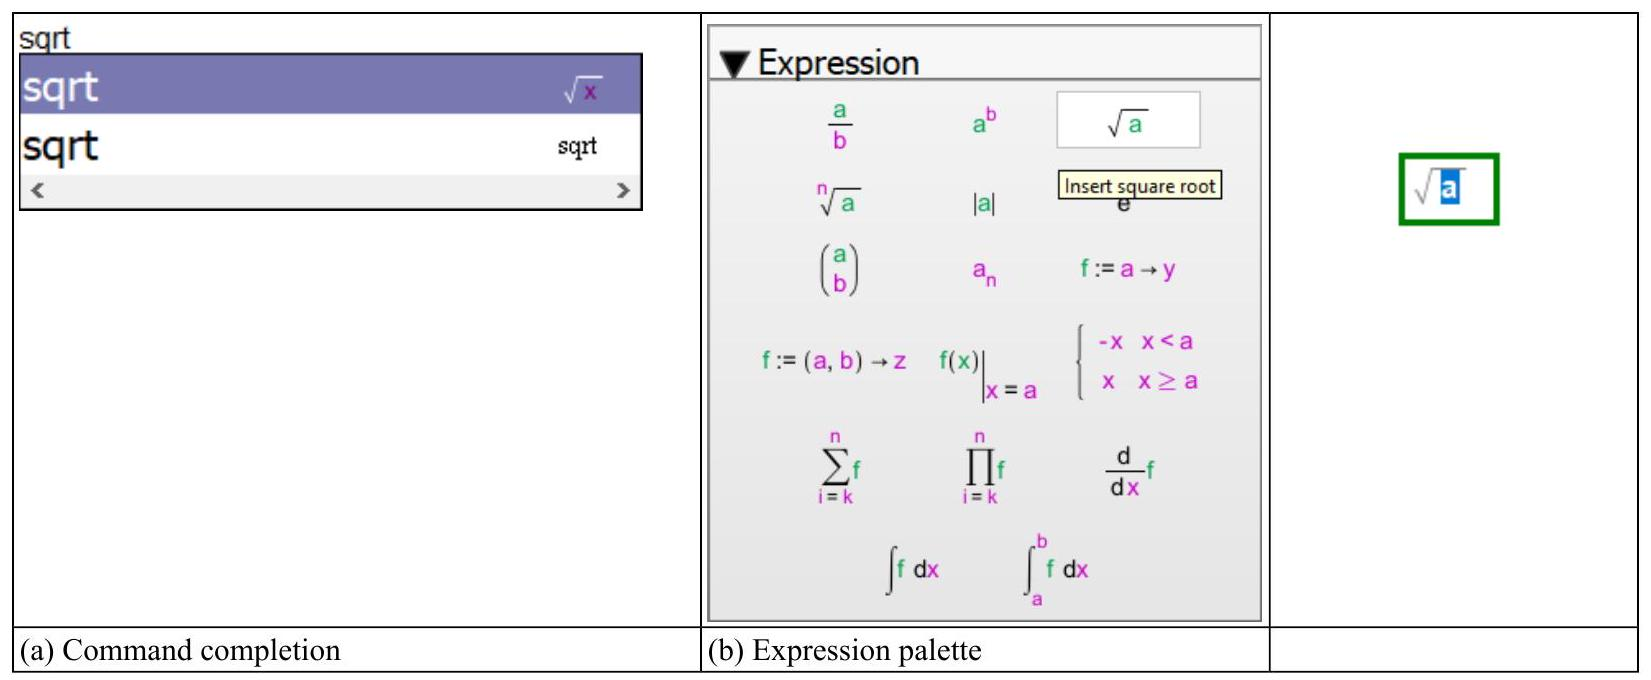
\includegraphics[max width=\textwidth]{2022_12_20_3e2ffe6ad124ec91ee5cg-18}
\end{center}

For more information on command completion, see Command Completion (page 31).

\subsection{Complex Numbers}
Imaginary numbers are entered with a number followed by the suffix $i$, with no multiplication between the two. For example, $2+2 \mathrm{i}$.

The unit complex number is created with 1i. You cannot just enter i for the unit complex number.

To create a symbolic multiplier on an imaginary number, you need to enter $\mathrm{x} * 1 \mathrm{i}$.

\subsection{Units}
\section{Entering Units}
You can enter units in several different ways.

\section{Units Palette}
You can enter units using the Units palette located in the Palettes pane on the left side of the Canvas. Click the desired unit (using the Dimensionality drop-down list to switch to different groups of units), or insert the unit placeholder (as illustrated in Figure 3.3) and overwrite the placeholder.

You may want to place a space between the number and the unit.

\begin{center}
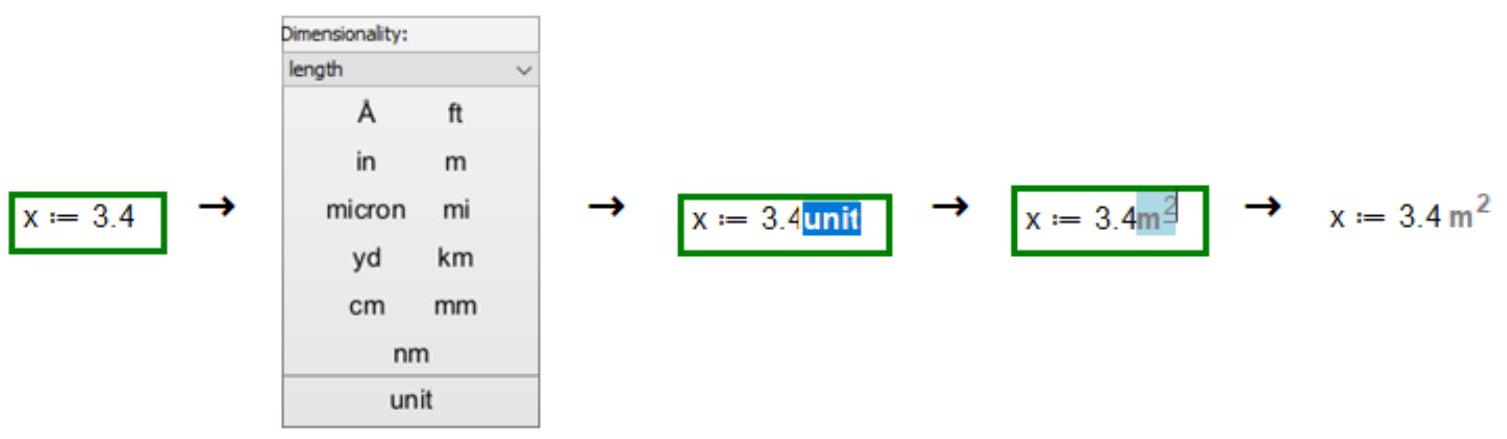
\includegraphics[max width=\textwidth]{2022_12_20_3e2ffe6ad124ec91ee5cg-18(1)}
\end{center}

Figure 3.3: Inserting a Unit with the Units Palette

\section{Unit function}
You can use the Unit 0 function to assign a unit.

$x:=3.4 \cdot \operatorname{Unit}\left(m^{2}\right)$

Figure 3.4: Using the Unit) function to assign a unit

\section{Keyboard shortcut}
Press $\mathbf{C t r l}+\mathbf{S h i f t}+\mathbf{U}$ to enter a unit placeholder. Then, replace the placeholder with the desired units.

$\mathrm{x}:=3.4$ unit

Figure 3.5: Using keyboard shortcuts to insert a unit placeholder

\section{Editing Existing Units}
Move the cursor onto the unit. When the unit has focus, it is highlighted by a light blue box. You can now change the unit.

Deleting all the characters in a unit placeholder will leave an empty placeholder one character in size. Deleting this empty placeholder will remove the unit placeholder entirely.

When the results of your calculations contains units, you can use the units formatting options in the Context Panel to rescale the units to units you'd prefer to see.

\begin{equation*}
\begin{aligned}
& \text { force }:=4.5 \mathrm{~N} \\
& \text { area }:=3.4 \mathrm{~cm}^{2} \\
& \text { stress }:=\frac{\text { force }}{\text { area }}=13235.294 \mathrm{~Pa}
\end{aligned}
\end{equation*}

\begin{center}
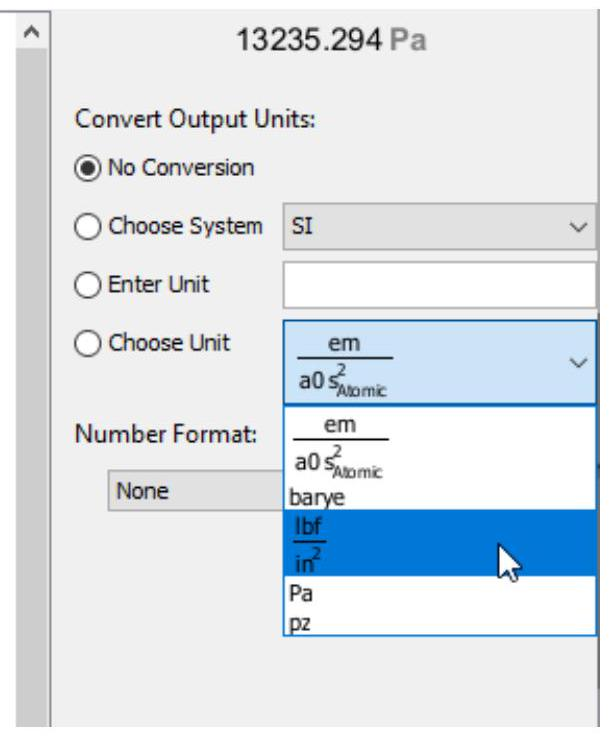
\includegraphics[max width=\textwidth]{2022_12_20_3e2ffe6ad124ec91ee5cg-19}
\end{center}

Figure 3.6: Convert output units

\subsection{Notes about Math Input}
\section{Numerical Evaluation and Accuracy}
Any purely numerical operations are evaluated to a floating-point approximation.

\begin{equation*}
\begin{aligned}
& \frac{1}{2}=0.500 \\
& \sqrt{2}=1.414 \\
& \sin (\sqrt{3} \cdot x)=\sin (1.732 \cdot x)
\end{aligned}
\end{equation*}

\section{Figure 3.7: Numerical operations}
The Digits environment variable controls the number of digits that Maple uses when making calculations with software floating-point numbers.

The default value of Digits is 10 . The value of Digits is changed with the assignment operator (e.g. Digits: $=15$ ).

Figure 3.8 illustrates the effect of changing digits from its default value of 10 to 15 on the evaluation of $2^{0.5}$. (Note that numeric formatting on the result of $2^{0.5}$ has been set to Fixed with 20 decimal places.)

\begin{equation*}
\begin{aligned}
& \text { Digits }:=10 \\
& 2^{0.5}=1.41421356200000000000 \\
& \text { Digits }:=15 \\
& 2^{0.5}=1.41421356237310000000
\end{aligned}
\end{equation*}

Figure 3.8: The effect of Digits on numerical accuracy

\section{Evaluation Order}
Maple Flow evaluates calculations from left-to-right, top-to-bottom (much like reading a page from a book). This means that downstream calculations only "see" assignments on the left or above. This is illustrated in Figure 3.9.

\begin{center}
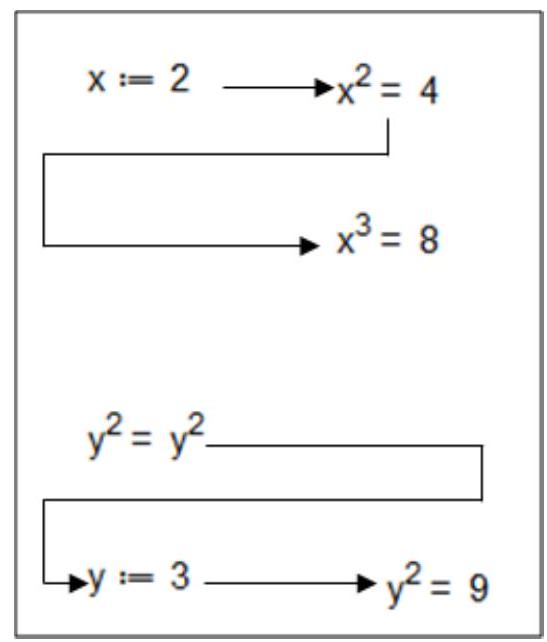
\includegraphics[max width=\textwidth]{2022_12_20_3e2ffe6ad124ec91ee5cg-20}
\end{center}

Figure 3.9: Spatial evaluation

You can change the evaluation order by moving math containers around.

\section{Nonexecutable Math and Disabling Evaluation}
You may want to enter nonexecuting math for documentation purposes. You can do this by entering math into a text container. For details, see Entering Math in a Text Container (page 16).

If you want to author content without any math evaluating in the Maple Flow worksheet, but eventually the math will be executed, you can temporarily disable evaluation.

To disable evaluation:

\begin{itemize}
  \item Click Turn evaluation off $(\overline{+}=$ ) on the toolbar. An indicator will appear at the top of the canvas indicating Evaluation Disabled.
\end{itemize}

To enable evaluation:

\begin{itemize}
  \item Click the icon again.
\end{itemize}

\section{Creating a Polished Document}
\subsection{Entering Text}
To enter text:

\begin{enumerate}
  \item Click in a blank part of the canvas.

  \item Press Space to create an empty text container. This will have a blue border.

  \item Type your text.

  \item Use the context toolbar to format your text.

\end{enumerate}

\begin{center}
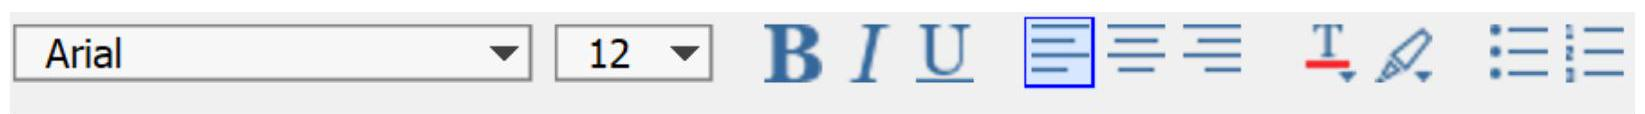
\includegraphics[max width=\textwidth]{2022_12_20_3e2ffe6ad124ec91ee5cg-22}
\end{center}

My first text

Figure 4.1: Entering and formatting text

\section{Entering Math in a Text Container}
You may want to enter nonexecuting math for documentation. You can do this by entering math into a text container.

To enter math in a text container:

\begin{enumerate}
  \item Anywhere inside a text container, press $\mathbf{C t r l}+\mathbf{R}$ to switch into math mode.

  \item Enter your math.

  \item If required, press $\mathbf{C t r l}+\mathbf{T}$ to return to text mode.

\end{enumerate}

\subsection{Math and Text Styling}
\section{Formatting the Content of Single Containers}
To change font, size, and font color, drag-select the content and use the context bar.

\section{Applying Background Color to a Math Container}
Math containers can also have a background color. This can be useful, for instance, to highlight a math container that contains the assignments for the variables that are used in the later calculations.

To apply a background color, right click on a math container.

\begin{center}
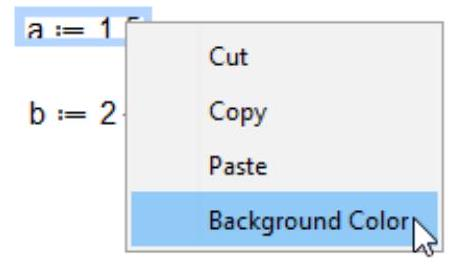
\includegraphics[max width=\textwidth]{2022_12_20_3e2ffe6ad124ec91ee5cg-22(1)}
\end{center}

Figure 4.2: Apply background color to a math container

The color selector dialog appears. Select a color.

\begin{center}
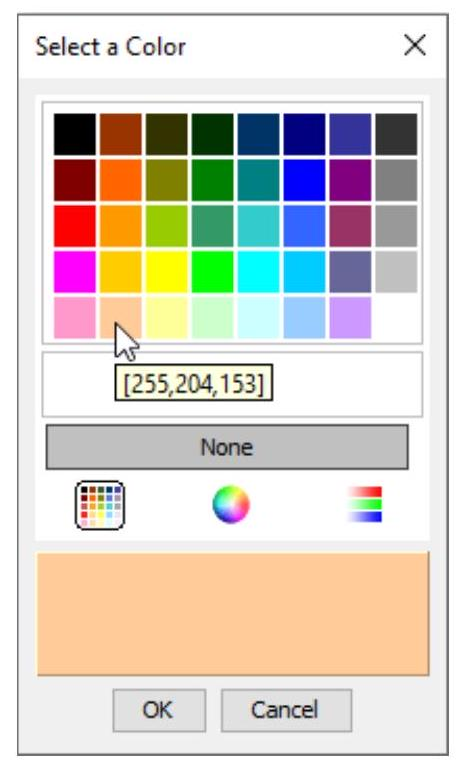
\includegraphics[max width=\textwidth]{2022_12_20_3e2ffe6ad124ec91ee5cg-23}
\end{center}

Figure 4.3: Select background color

Figure 4.4 shows the result of using background color on the math containers that define two assignments.

\begin{center}
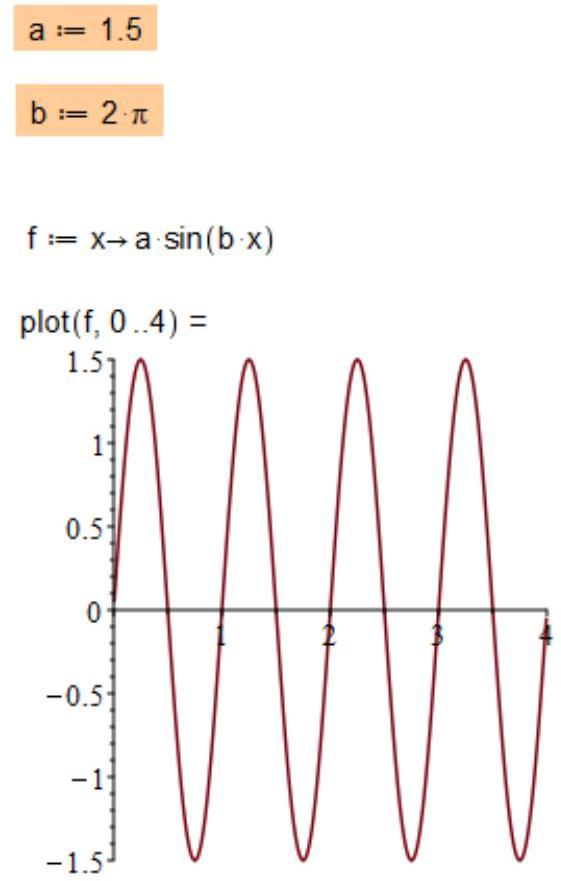
\includegraphics[max width=\textwidth]{2022_12_20_3e2ffe6ad124ec91ee5cg-23(1)}
\end{center}

Figure 4.4: A math container with background color

For information on creating plots, see Plots (page 30).

\section{Applying and Changing Styles}
The style drop-down list contains several formatting styles for text and math.

\begin{center}
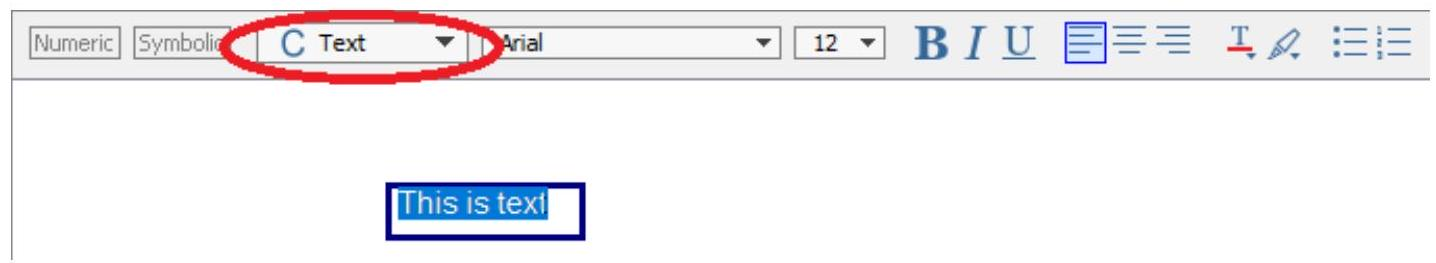
\includegraphics[max width=\textwidth]{2022_12_20_3e2ffe6ad124ec91ee5cg-24}
\end{center}

Figure 4.5: The Styles drop-down list

By default:

\begin{itemize}
  \item Text is given the Text style.

  \item Math input is given the 2D Math style.

  \item Math output is given the 2D Output style.

\end{itemize}

You can apply other styles with the other entries (such as the Title style for text). You will need to drag-select the content of the container and pick the appropriate style.

Use the Format $>$ Styles menu to change the typeface of the pre-defined styles.

Use the Format > Manage Style Sets menu to:

\begin{itemize}
  \item Export and save the active style set.

  \item Load and apply an existing style set.

\end{itemize}

\subsection{Using Sections}
You can use sections to organize your document.

To create a section:

\begin{enumerate}
  \item Select Insert $>$ Section.
\end{enumerate}

If you select some content and then use Insert $>$ Section, the selection will be enclosed in the section.

\begin{enumerate}
  \setcounter{enumi}{1}
  \item Enter a title for the section. You can modify the font/style for the title.
\end{enumerate}

To change the size of the section, you can drag the bottom boundary line. If you drag the section boundary past additional content, the section now encloses that content.

To collapse a section:

\begin{itemize}
  \item Click the collapse button (-).
\end{itemize}

To expand a section:

\begin{itemize}
  \item Click the expand button ( $)$.
\end{itemize}

Figure 4.6 shows an example of a Maple Flow worksheet with sections. The first section is collapsed and the second section is expanded.

\begin{center}
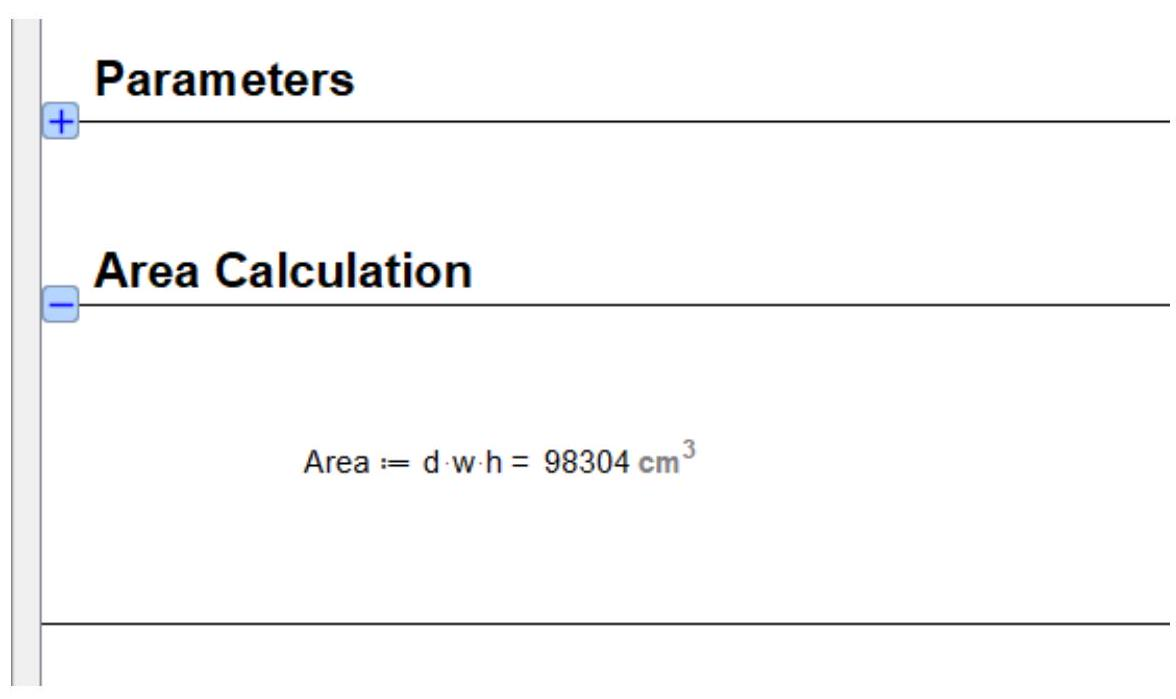
\includegraphics[max width=\textwidth]{2022_12_20_3e2ffe6ad124ec91ee5cg-25}
\end{center}

Figure 4.6: Sections in a worksheet

Evaluation order still applies as it normally does, and content in a section is evaluated even if a section is collapsed.

\section{Controlling the Display of Sections}
You can edit a section title by clicking in the text box for the title, or by clicking on the top boundary line.

Tip: If a section does not have a title, click on the top boundary line. This opens the title text box for editing.

You can control the display of sections using Format $>$ Section Style. From this dialog, you can

\begin{itemize}
  \item Control whether to display the top and bottom boundary lines.

  \item Control whether boundaries are displayed on only the left-most page.

  \item Specify margins.

  \item Specify boundary line thickness.

  \item Specify boundary line color.

  \item Specify boundary opacity.

  \item Control whether to display the expand button.

\end{itemize}

Note that if the section style is set up so the expand/collapse button is not displayed, you can expand or collapse a section by doing one of the following:

\begin{itemize}
  \item Click the left most part of the top section boundary line

  \item Double-click anywhere along the top section boundary line.

\end{itemize}

For information on controlling the display of sections when printing or exporting to PDF, see Printing a Worksheet with Sections (page 33).

\section{Removing a Section}
To remove a section:

\begin{itemize}
  \item Use Edit > Remove Section. The content remains in the canvas, and the section boundaries are removed.
\end{itemize}

\subsection{Hide Commands}
When creating a document, you have control over the display of the content of math containers. You can hide the input expression and just show the resulting output by right-clicking on the math container and selecting Hide commands from the context menu.

In the case of an assignment, you can select either Hide commands or Hide commands and name.

\begin{equation*}
\begin{aligned}
& b:=15 \\
& a:=\frac{b}{5}=3 \\
& \text { sol: }=\text { fsolve }(\ln a(a \cdot x)+a=x \quad x)=n \cap 17 \\
& \text { Cut } \\
& \text { Copy } \\
& \text { Paste }
\end{aligned}
\end{equation*}

Hide commands

Hide commands and name

Background Color

Figure 4.7: Hide commands

There is an option to display a visual indicator for math containers that have hidden commands. To enable this setting, select View > Visual Indicators. When Visual Indicators is selected, a math container with hidden commands is drawn with a gray circle at the top left corner.

\begin{equation*}
\begin{aligned}
& b:=15 \\
& a:=\frac{b}{5}=3 \\
& \text { sol }=0.017
\end{aligned}
\end{equation*}

Figure 4.8: Marker indicates hidden command

To show the command again, right-click and select Show commands from the context menu.

\subsection{Including Images and Drawings}
You can insert images into your worksheet using Insert > Image.

You can also use the drawing tools on an image.

\section{Drawing Tools}
To view the drawing tools, select an image in your Maple Flow worksheet. The Context toolbar displays the Drawing toolbar.

\begin{center}
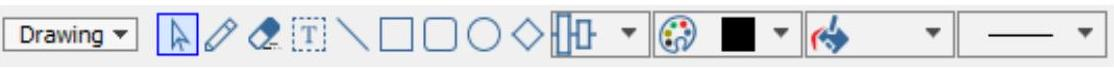
\includegraphics[max width=\textwidth]{2022_12_20_3e2ffe6ad124ec91ee5cg-26}
\end{center}

\section{Figure 4.9: Drawing Toolbar}
The tools include the following: selection tool, pencil (free style drawing), eraser, text insert, straight line, rectangle, rounded rectangle, oval, diamond, alignment tool, drawing outline tool, drawing fill tool, and line style tool. Tip: For the text, line, rectangle, round rectangle, oval, and diamond tools,

\begin{itemize}
  \item Click once on the toolbar icon to insert that type of object into the drawing. The tool is activated. For example, $\sqrt{3}$

  \item Click twice on the toolbar icon to insert multiple objects of the same type without having to reselect the tool.

\end{itemize}

The icon is highlighted yellow. For example, . The tool remains activated until you select another toolbar icon.

Text

\begin{center}
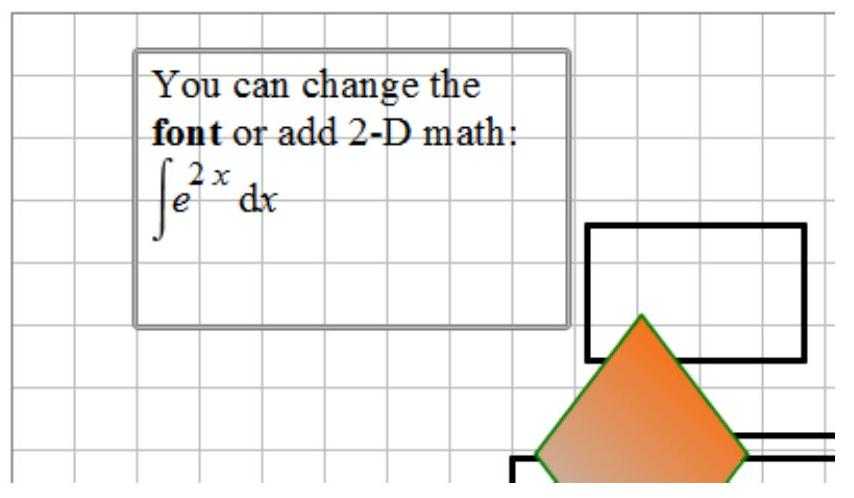
\includegraphics[max width=\textwidth]{2022_12_20_3e2ffe6ad124ec91ee5cg-27}
\end{center}

To insert text in the drawing canvas:

\begin{enumerate}
  \item Click the text icon (T).

  \item Click in the drawing canvas (on the image). A text box appears.

  \item Enter text and modify font as necessary using the toolbar font and font size drop-down lists. Include math in the text box in the same way you include math in a text container. See Entering Math in a Text Container (page 16).

  \item Optional. Select a fill color for a text box or select the line color for the border in the same way it is done for objects.

\end{enumerate}

\section{Lines - Straight, Resizing, Adding Arrows}
\section{Drawing Straight Lines}
\section{To draw a straight line:}
\begin{enumerate}
  \item Click the straight line icon $(\backslash)$.

  \item (Optional) From the

\end{enumerate}

\begin{center}
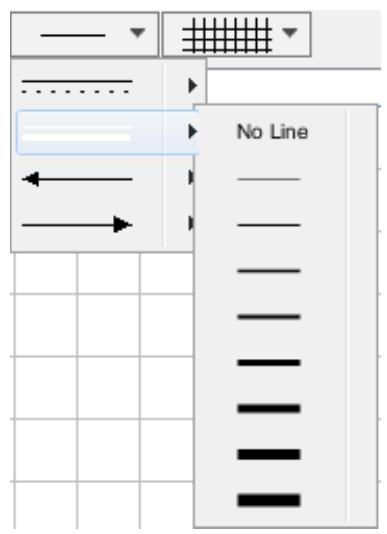
\includegraphics[max width=\textwidth]{2022_12_20_3e2ffe6ad124ec91ee5cg-28}
\end{center}

\begin{enumerate}
  \setcounter{enumi}{2}
  \item In the canvas, click and drag the mouse. A straight line is drawn.

  \item To complete the line, click the mouse twice or press Enter. The drawing feature switches to the Selection tool.

  \item You can draw more than one connected line; to complete your drawing, click the mouse twice, press Enter, or bring the end of the last line back to the start of the first line.

  \item To remove the last point drawn, press Esc.

\end{enumerate}

\section{Drawing a Line that Snaps to Vertical, Horizontal, or a 45 Degree Angle}
To draw a line that snaps to an orientation that is a multiple of 45 degrees:

\begin{enumerate}
  \item Click the straight line icon.

  \item In the canvas, click and drag the mouse.

  \item Press and hold the Shift key to snap to a 45 degree increment.

  \item To complete the line, click the mouse twice or press Enter.

\end{enumerate}

\section{Drawing a Line that is Attached to a Shape}
\section{To draw a line that is attached to a shape in the drawing canvas:}
If you have inserted a shape in the canvas, you can draw a line that is automatically attached to that shape.

\begin{enumerate}
  \item Click the straight line icon.

  \item Press and hold the Ctrl key, and, in the canvas, hover your mouse cursor over the existing shape to which you want to attach the line. The shape is highlighted in green.

  \item To draw the line, click and drag the mouse.

  \item To complete the line, click the mouse twice or press Enter. The drawing feature switches to the Selection tool.

\end{enumerate}

\section{Resizing Lines}
\section{To resize objects drawn with straight lines:}
\begin{enumerate}
  \item Select the line to be resized using the selection tool.

  \item With the mouse pointer over a grab box, click and drag the line to increase or decrease its size.

  \item Release the mouse button.

\end{enumerate}

\begin{center}
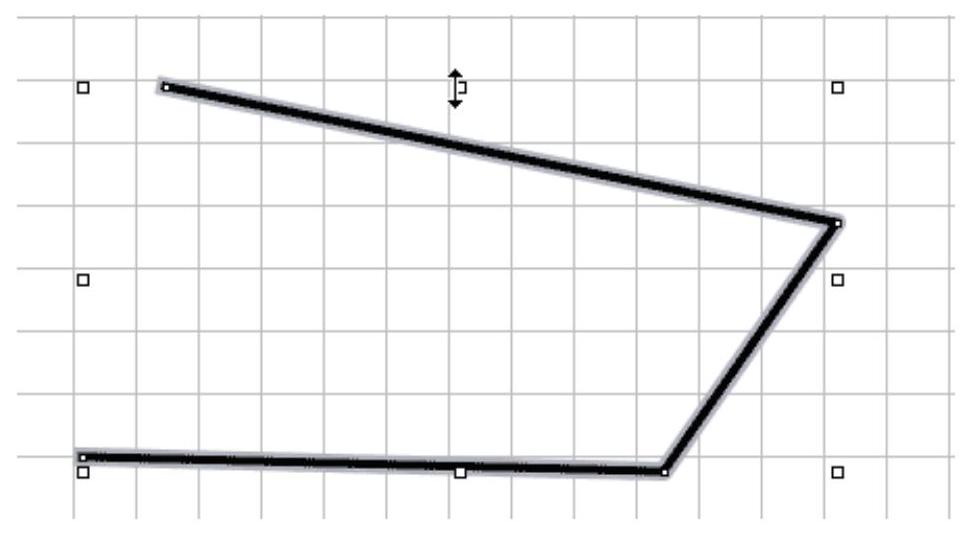
\includegraphics[max width=\textwidth]{2022_12_20_3e2ffe6ad124ec91ee5cg-29}
\end{center}

\section{Changing Vertices of Lines}
\section{To change vertices of drawn lines in the canvas:}
When an object is selected, grab boxes and nodes at the vertices are displayed.

\begin{center}
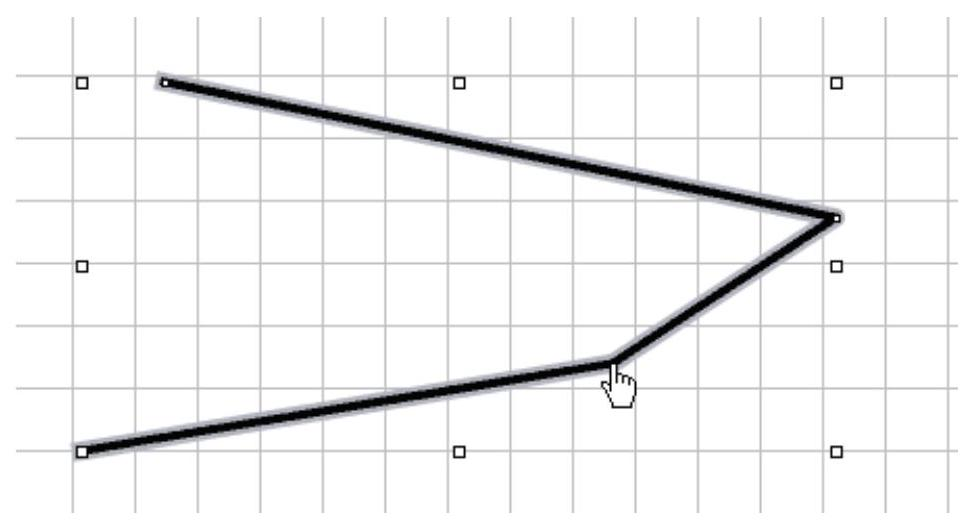
\includegraphics[max width=\textwidth]{2022_12_20_3e2ffe6ad124ec91ee5cg-29(1)}
\end{center}

\begin{enumerate}
  \item Click a node and drag the mouse to the desired point, thereby changing the vertex position.

  \item Release the mouse.

\end{enumerate}

\section{Changing the Line Style}
\section{To change the style of drawn lines:}
You can change the line style, thickness, and arrow points of a line either when it is drawn or afterwards.

\begin{enumerate}
  \item Select a line using the selection tool.

  \item From the $\square$ menu, select a line style, thickness, or arrow direction and shape.

\end{enumerate}

\begin{center}
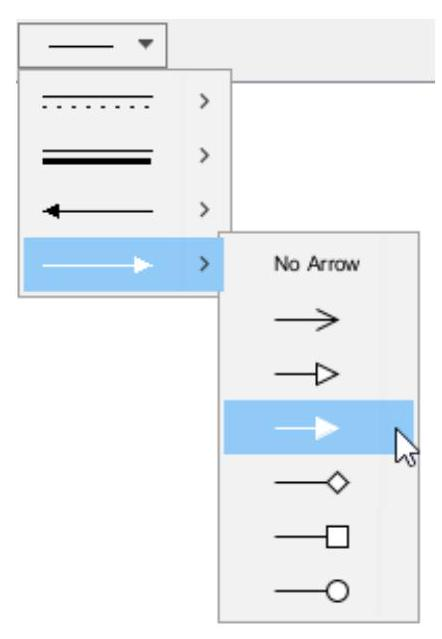
\includegraphics[max width=\textwidth]{2022_12_20_3e2ffe6ad124ec91ee5cg-30}
\end{center}

The selected change is automatically applied to the straight line.

For example, a straight, thick line will have a solid arrow on the right end after clicking on the menu item displayed above.

\begin{center}
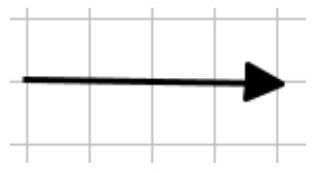
\includegraphics[max width=\textwidth]{2022_12_20_3e2ffe6ad124ec91ee5cg-30(1)}
\end{center}

\section{Rotating Images or Rotating Objects in a Drawing}
You can rotate an image, or an object in a drawing. The process is the same.

\begin{center}
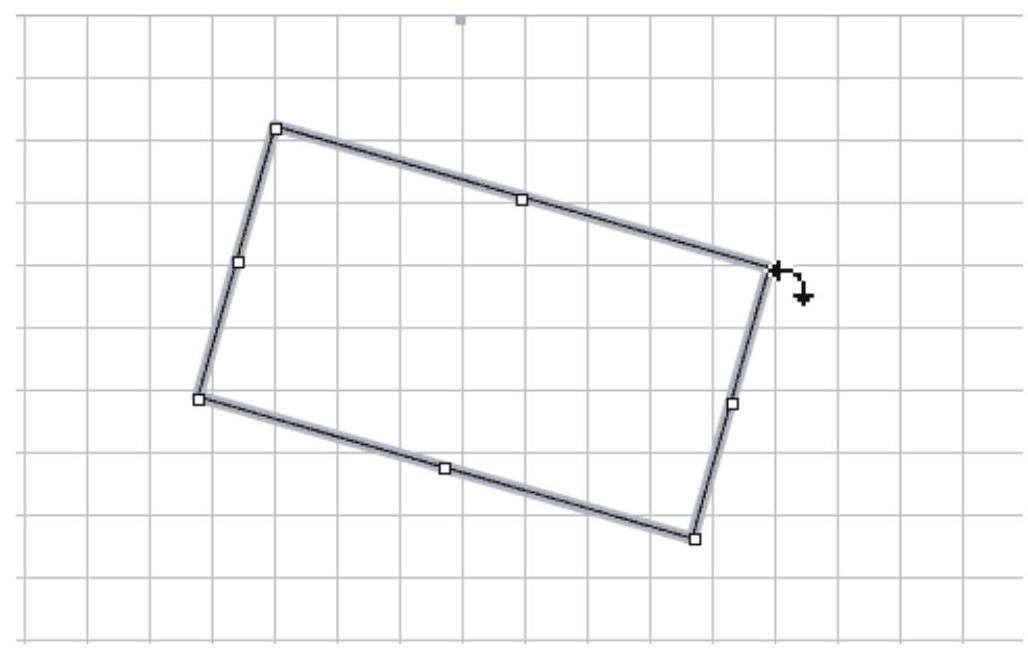
\includegraphics[max width=\textwidth]{2022_12_20_3e2ffe6ad124ec91ee5cg-30(2)}
\end{center}

To rotate an object:

\begin{enumerate}
  \item Select the object. The vertices of the object are designated by grab boxes.

  \item Place the cursor at one of the vertices.

  \item Press Ctrl. The rotate icon is displayed.

  \item While pressing Ctrl, click the mouse and drag. The object rotates. Release the mouse once the object is positioned as you want.

\end{enumerate}

\section{Color Selection Dialog}
The drawing outline tool, drawing fill tool, and canvas properties tool allow you to select colors for shapes, lines, and the canvas grid lines. Choose a color by using one of the following tools in the color selection dialog:

\begin{center}
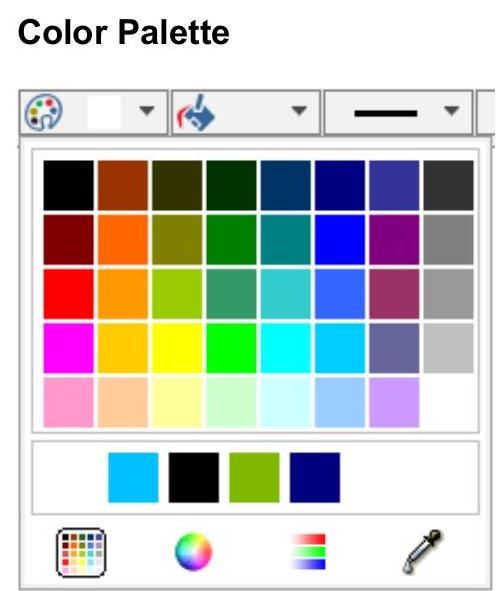
\includegraphics[max width=\textwidth]{2022_12_20_3e2ffe6ad124ec91ee5cg-31}
\end{center}

To select a color, click a color from a palette of pre-defined colors.

The last five colors that you select are displayed in the box below the color swatches. If you want to view the RGB values of a particular color, hover your mouse cursor over a color swatch.

\section{Color Wheel}
\begin{center}
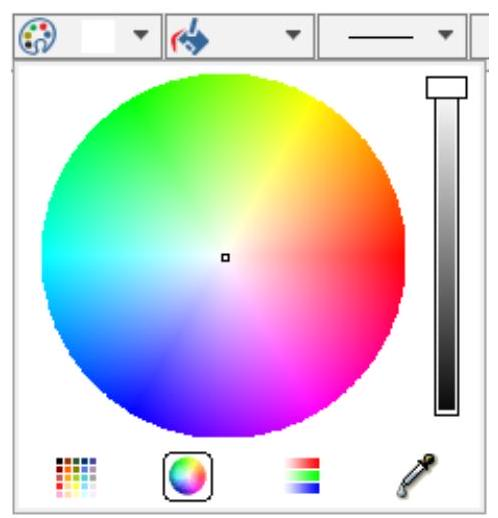
\includegraphics[max width=\textwidth]{2022_12_20_3e2ffe6ad124ec91ee5cg-31(1)}
\end{center}

\section{To select a color:}
\begin{enumerate}
  \item Move the slider beside the color wheel to display a range of colors.

  \item To select a color, click a point in the color wheel.

\end{enumerate}

\section{Color Value Sliders}
\begin{center}
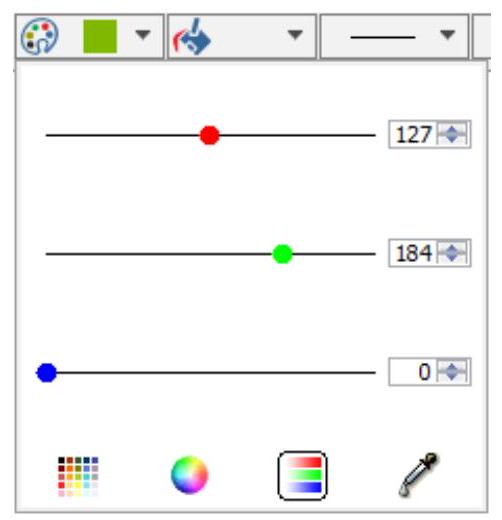
\includegraphics[max width=\textwidth]{2022_12_20_3e2ffe6ad124ec91ee5cg-32}
\end{center}

To select a color, specify the RGB values of the color by moving the sliders. Alternatively, you can use the spinners to scroll to certain values or type the values directly in the fields. For each RGB value, you can specify a number from 0 to 225 .

\begin{center}
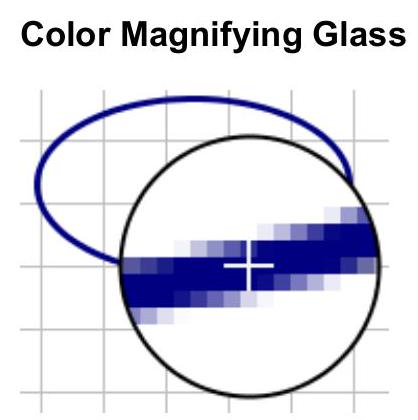
\includegraphics[max width=\textwidth]{2022_12_20_3e2ffe6ad124ec91ee5cg-32(1)}
\end{center}

To select a color:

\begin{enumerate}
  \item Select the eye dropper icon ( ).

  \item Hover the color magnifying glass over an area on your screen that displays the color you want to select.

  \item Using your mouse cursor, in the circle, click a point that displays the color.

\end{enumerate}

To cancel your selection, right-click the circle.

\section{Pencil Tool - Free Form drawing}
To draw with the pencil tool in the canvas:

\begin{enumerate}
  \item From the drawing icons, select the pencil tool icon ( ).

  \item Click and drag your mouse in the canvas to draw lines. Release the mouse to complete the drawing.

\end{enumerate}

\section{Selection Tool - How and When to Use}
To select items in the canvas use the selection tool .

You can use the selection tool to select a single object or a group of objects. To select a group of objects:

Using the selection tool, click and drag the mouse around the items to be grouped. Release the mouse button. The items are temporarily grouped.

Apply formatting as desired, for example by using the alignment tools in the Drawing toolbar. To temporarily switch to the selection tool (when using another tool), press and hold the Tab key (Command, Mac). You can move and resize objects. When you release the Tab key, the tool will revert to its previous setting. This allows you to tweak something you just drew.

\section{Filling Objects - Solid or Gradient Fill Colors}
\section{Filling an Object with a Solid Color}
To fill an object with a solid color:

\begin{enumerate}
  \item Select the object in the canvas.

  \item From ther $\quad$ menu, select the solid fill style at the top (next to None).

  \item From the same menu, click the left color bar at the bottom, and select a color from the color palette.

\end{enumerate}

\begin{center}
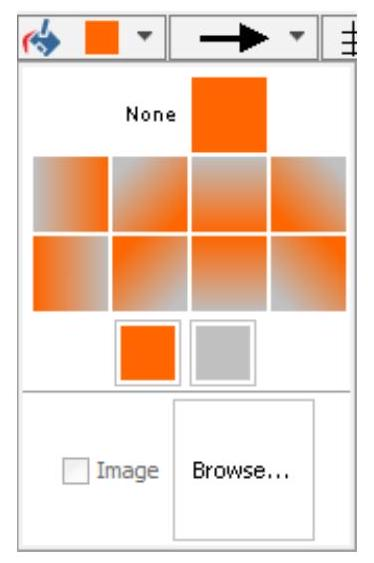
\includegraphics[max width=\textwidth]{2022_12_20_3e2ffe6ad124ec91ee5cg-33}
\end{center}

\begin{enumerate}
  \setcounter{enumi}{3}
  \item To change the line color, select a color from the $\square$ menu.
\end{enumerate}

\begin{center}
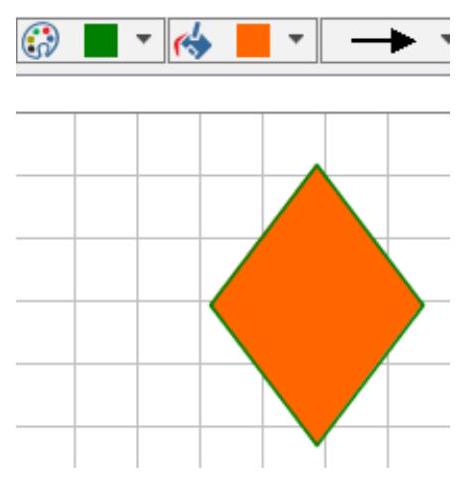
\includegraphics[max width=\textwidth]{2022_12_20_3e2ffe6ad124ec91ee5cg-33(1)}
\end{center}

\section{Filling an Object with a Gradient Color}
\section{To fill an object with a gradient color:}
\begin{enumerate}
  \item Select the object in the canvas.

  \item From the $\quad \nabla$ menu, select one of the gradient fill styles, the square icons.

  \item From the same menu, click the left and right color bars at the bottom to select a color from the color palette for each part of the gradient.

\end{enumerate}

\begin{center}
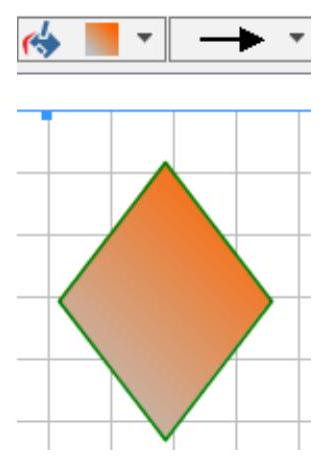
\includegraphics[max width=\textwidth]{2022_12_20_3e2ffe6ad124ec91ee5cg-34}
\end{center}

See below for instructions on filling an object with an image.

\subsection{Creating Hyperlinks}
You can add a hyperlink to a worksheet that links to another Maple Flow worksheet, a webpage, and more.

To insert a hyperlink:

\begin{enumerate}
  \item In a text container, select Insert>Hyperlink. The Hyperlink Properties dialog opens.

  \item For the Link Text field, enter the text to be shown.

  \item Select the link type.

  \item For the Target field, enter the destination. Note that you have to save your document if you want to use a relative path.

  \item Optionally, you can add a hyperlink tooltip.

\end{enumerate}

You can also create a hyperlink by selecting some text and using the Format $>$ Convert $>$ Hyperlink menu item.

To edit the hyperlink properties, right-click the hyperlink and select Hyperlink Properties from the context menu.

You can create a hyperlink to a Maple Flow help page. For example, setting Type to Help Topic and Target to solve creates a link to the solve help page.

\begin{center}
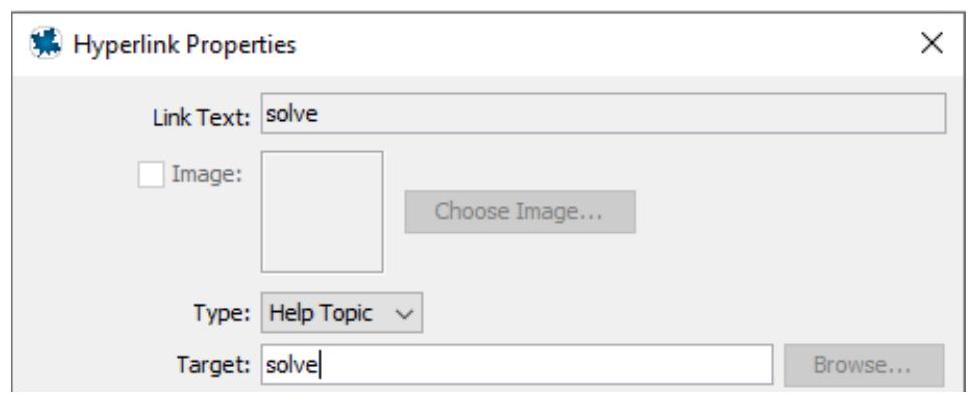
\includegraphics[max width=\textwidth]{2022_12_20_3e2ffe6ad124ec91ee5cg-34(1)}
\end{center}

Figure 4.10: Help Topic Hyperlink

In addition to hyperlinks, your worksheet can contain shortcut components, which are clickable image links. The default look of a shortcut is shown in Figure 4.11, but you can change the image used. The Application Gallery in Maple Flow uses shortcuts.

\begin{center}

\includegraphics[max width=\textwidth]{2022_12_20_3e2ffe6ad124ec91ee5cg-35}
\end{center}

Shortcut

Figure 4.11: Shortcut

To insert a shortcut:

\begin{enumerate}
  \item Click on the canvas.

  \item Select Insert $>$ Shortcut. A shortcut component is inserted at the cursor.

  \item To edit the shortcut properties, select the shortcut component, and in the Context Panel the shortcut properties are available.

\end{enumerate}

\begin{center}
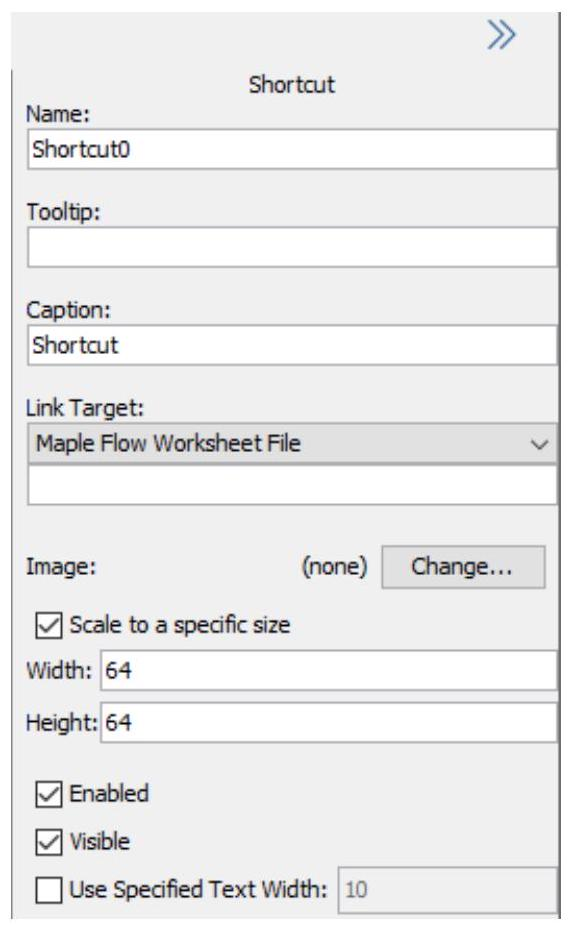
\includegraphics[max width=\textwidth]{2022_12_20_3e2ffe6ad124ec91ee5cg-35(1)}
\end{center}

Figure 4.12: Shortcut Properties

\begin{enumerate}
  \setcounter{enumi}{3}
  \item Specify a caption, which appears below the image. Optionally, add a tooltip. Note: The Name field is used by Maple Flow to identify the component. The caption is what is visible.

  \item Specify a link target. You can link to a Maple Flow worksheet or URL. You can also use the Shortcut to open a blank Maple Flow worksheet,

  \item If desired, change the image.

\end{enumerate}

\section{Further Tools: Mathematical Functions, Programming, and Plots}
\subsection{Mathematical Functions}
\section{Maple Functions}
Maple Flow is built on top of the Maple programming language. You can use most Maple functions in Maple Flow.

Maple package functions are used in the long form. For example, SignalProcessing:-FFT(). Note: Use of the with() command to load packages is not supported.

The Maple programming language is described in the Maple online help: \href{http://www.maplesoft.com/support/help}{http://www.maplesoft.com/support/help}.

\section{Unsupported Maple Keywords, Commands, and Packages}
As noted above, the with 0 command is not supported, and instead package commands should be called using the long form of their name. In addition, some Maple keywords, commands, and packages are not supported. The following are some examples, but not a complete list.

The assume command is not supported (use assuming instead). Some keywords, such as read and save, are not supported.

These Maple packages are not supported:

\begin{itemize}
  \item Physics

  \item Tolerances

  \item DocumentTools

  \item Typesetting

\end{itemize}

Procedures can only be defined in the Code Editor. See Code Editor (page 31).

\subsection{Plots}
You can create a plot with the Maple language plot command. A simple example is given in Figure 5.1.

\begin{center}
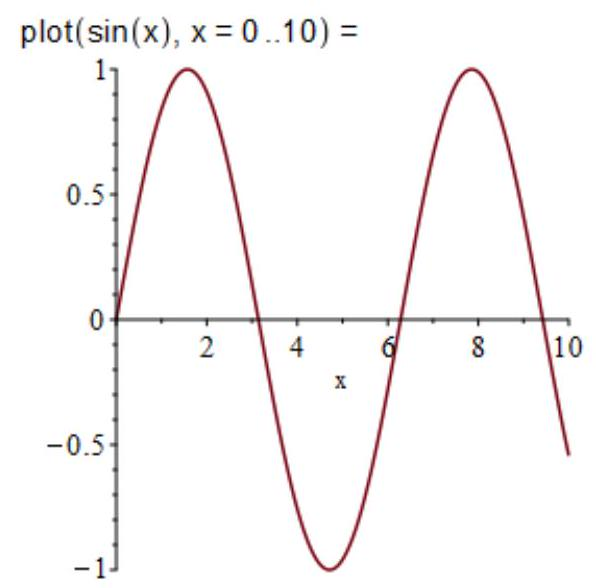
\includegraphics[max width=\textwidth]{2022_12_20_3e2ffe6ad124ec91ee5cg-36}
\end{center}

Figure 5.1: A simple plot using a Maple plot command

Plots can be rotated in the same way that drawings are rotated. To rotate the plot:

\begin{enumerate}
  \item Select the plot container with the selection tool. The vertices of the plot container are designated by grab boxes.

  \item Place the cursor at one of the vertices.

  \item Press Ctrl. The rotate icon is displayed.

  \item While pressing Ctrl, click the mouse and drag. The plot container rotates. Release the mouse once the object is positioned as you want.

\end{enumerate}

\subsection{Command Completion}
Maple Flow offers a dialog for command completion. Maple Flow suggests commands and parameters that complete what you have already entered.

The command completion dialog is initiated by pressing Esc or Ctrl + Space.

fs

fscanf

fscr $\quad f$

fsolve $\quad$ fsolve

fsolve $\quad$ fsolve(eqn)

fsolve (equation set) $\quad$ fsolve( ( eqn 1, eqn $2, \ldots\})$

fsolve (equation set, complex solutions) fsolve( (eann 1, eqn $2, \ldots\}$, complex')

Figure 5.2: Command completion window

\subsection{Code Editor}
The Code Editor lets you write Maple procedures to use in a Maple Flow canvas. To learn how to write a Maple procedure, read the online Maple Programming Guide:

\href{https://www.maplesoft.com/support/help/Maple/view.aspx?path=ProgrammingGuide/Contents}{https://www.maplesoft.com/support/help/Maple/view.aspx?path=ProgrammingGuide/Contents}

To view the code editor, click the Code Editor button on the main toolbar, as illustrated in Figure 5.3. Alternatively, from the Edit menu, select Code.

\begin{center}

\includegraphics[max width=\textwidth]{2022_12_20_3e2ffe6ad124ec91ee5cg-37}
\end{center}

Figure 5.3: Code Editor button on main toolbar

Note: You can only enter proc definitions in the code editor. That is, your code should be in the form:

FirstProc: $=$ proc $(\ldots) \quad \ldots$ end proc;

NextProc:=proc (...) $\ldots$ end proc;

To define the procedure, enclose a sequence of statements between proc(...) and end proc statements, and specify the parameter name(s) in the parentheses after the proc statement. For example, a simple definition for a procedure that takes one parameter and returns the square of the parameter is:

MyProc: $=\operatorname{proc}(\mathrm{x}) \mathrm{x}^{\wedge} 2$; end proc;

\section{Printing and Exporting to PDF}
\subsection{Print Extents}
Selecting View $>$ Print Extents displays dashed horizontal and vertical lines. These indicate the extents of a printable page, taking into account the chosen page size, margins and headers/footers. Pages are printing column-by-column.

\begin{center}
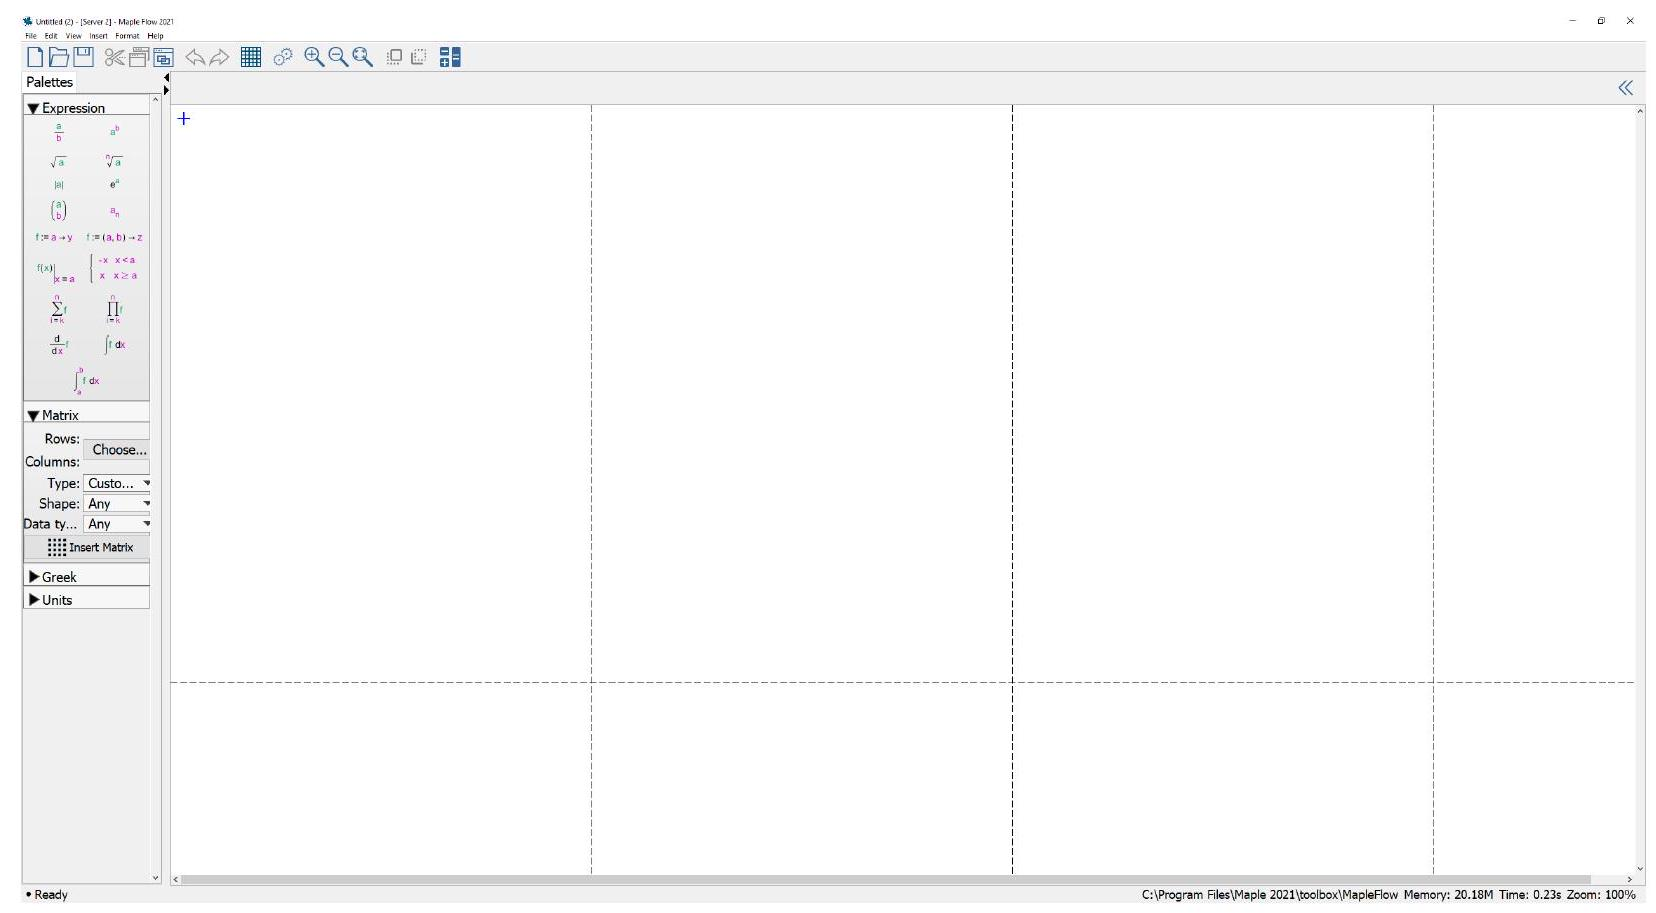
\includegraphics[max width=\textwidth]{2022_12_20_3e2ffe6ad124ec91ee5cg-38}
\end{center}

Figure 6.1: Print extents

The on-screen positioning and size of math, text, plots and images will be reflected in the printed page or exported PDF.

\subsection{Headers/Footers}
The Insert $>$ Header Footer menu lets you specify a header and/or footer. This will be seen in the printed page or exported PDF, but not in the working environment.

\begin{center}
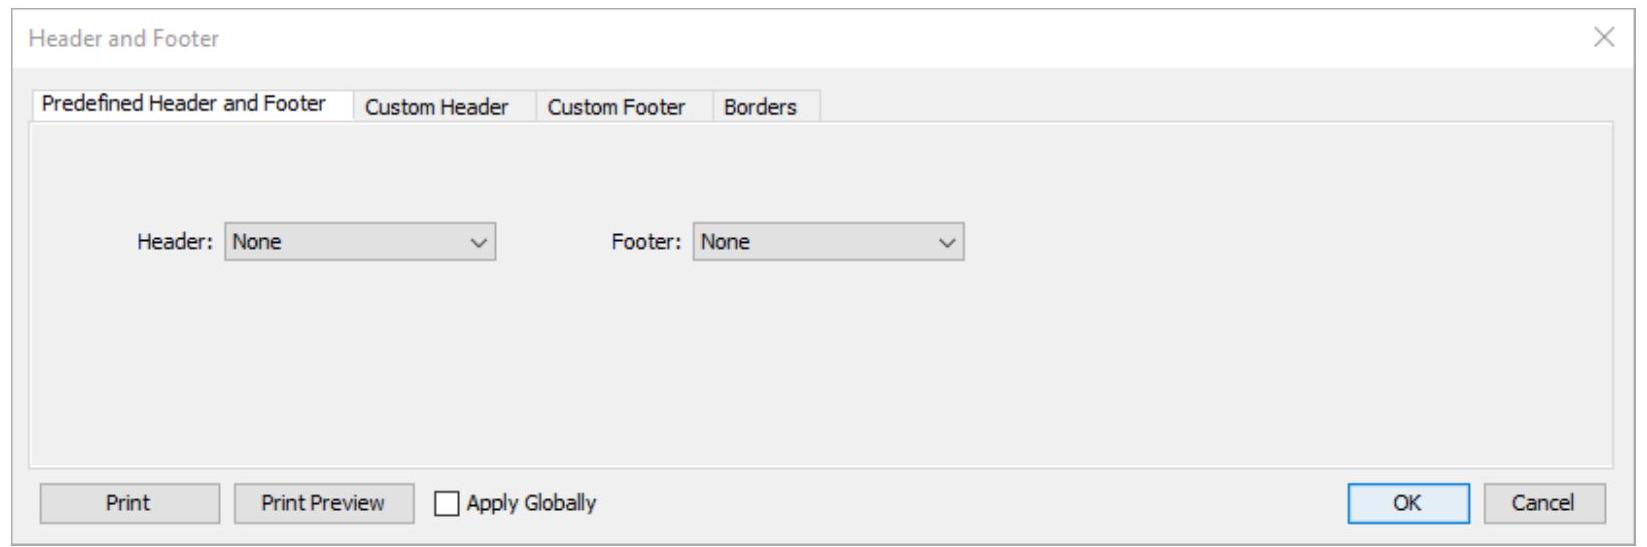
\includegraphics[max width=\textwidth]{2022_12_20_3e2ffe6ad124ec91ee5cg-38(1)}
\end{center}

Figure 6.2: Inserting Headers and Footers

\subsection{Page Setup and Print Preview}
The File $>$ Page Setup menu lets you change the page size, orientation, and margins, for printing.

\begin{center}
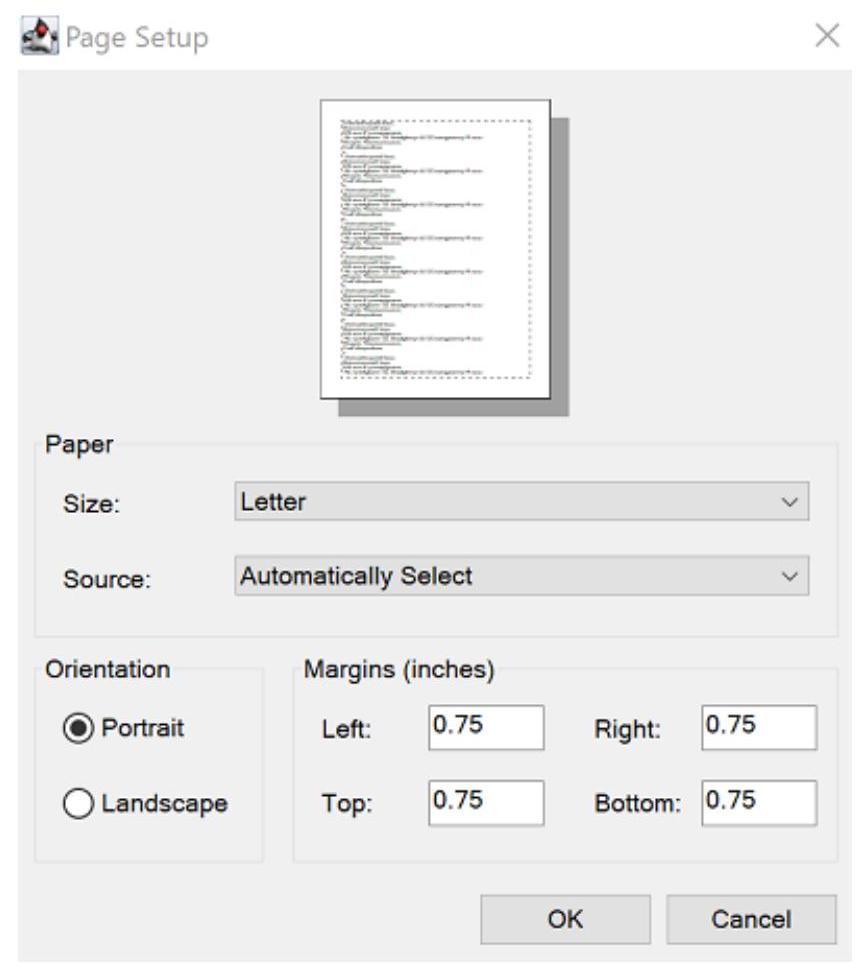
\includegraphics[max width=\textwidth]{2022_12_20_3e2ffe6ad124ec91ee5cg-39}
\end{center}

Figure 6.3: Page Setup

The File $>$ Print Preview menu lets you preview the printed page or exported PDF.

\subsection{Export to PDF}
To export the canvas to a PDF, click Print $>$ Export.

\subsection{Printing a Worksheet with Sections}
Whether printing or exporting to PDF, if your Maple Flow worksheet has sections, you can select how it is printed.

When you select Print or Print Preview, the Section Options for Print and PDF dialog opens. Select one of the following:

\begin{itemize}
  \item Print/export document with all sections expanded.

  \item Print/export document keeping sections exactly as shown on-screen.

\end{itemize}

If you selected the first option, in addition, specify whether to print the section boundary markers.

For more information on controlling the display of sections, see Controlling the Display of Sections (page 19).

\section{Keyboard Shortcuts}
Table 7.1: Keyboard shortcuts

\begin{center}
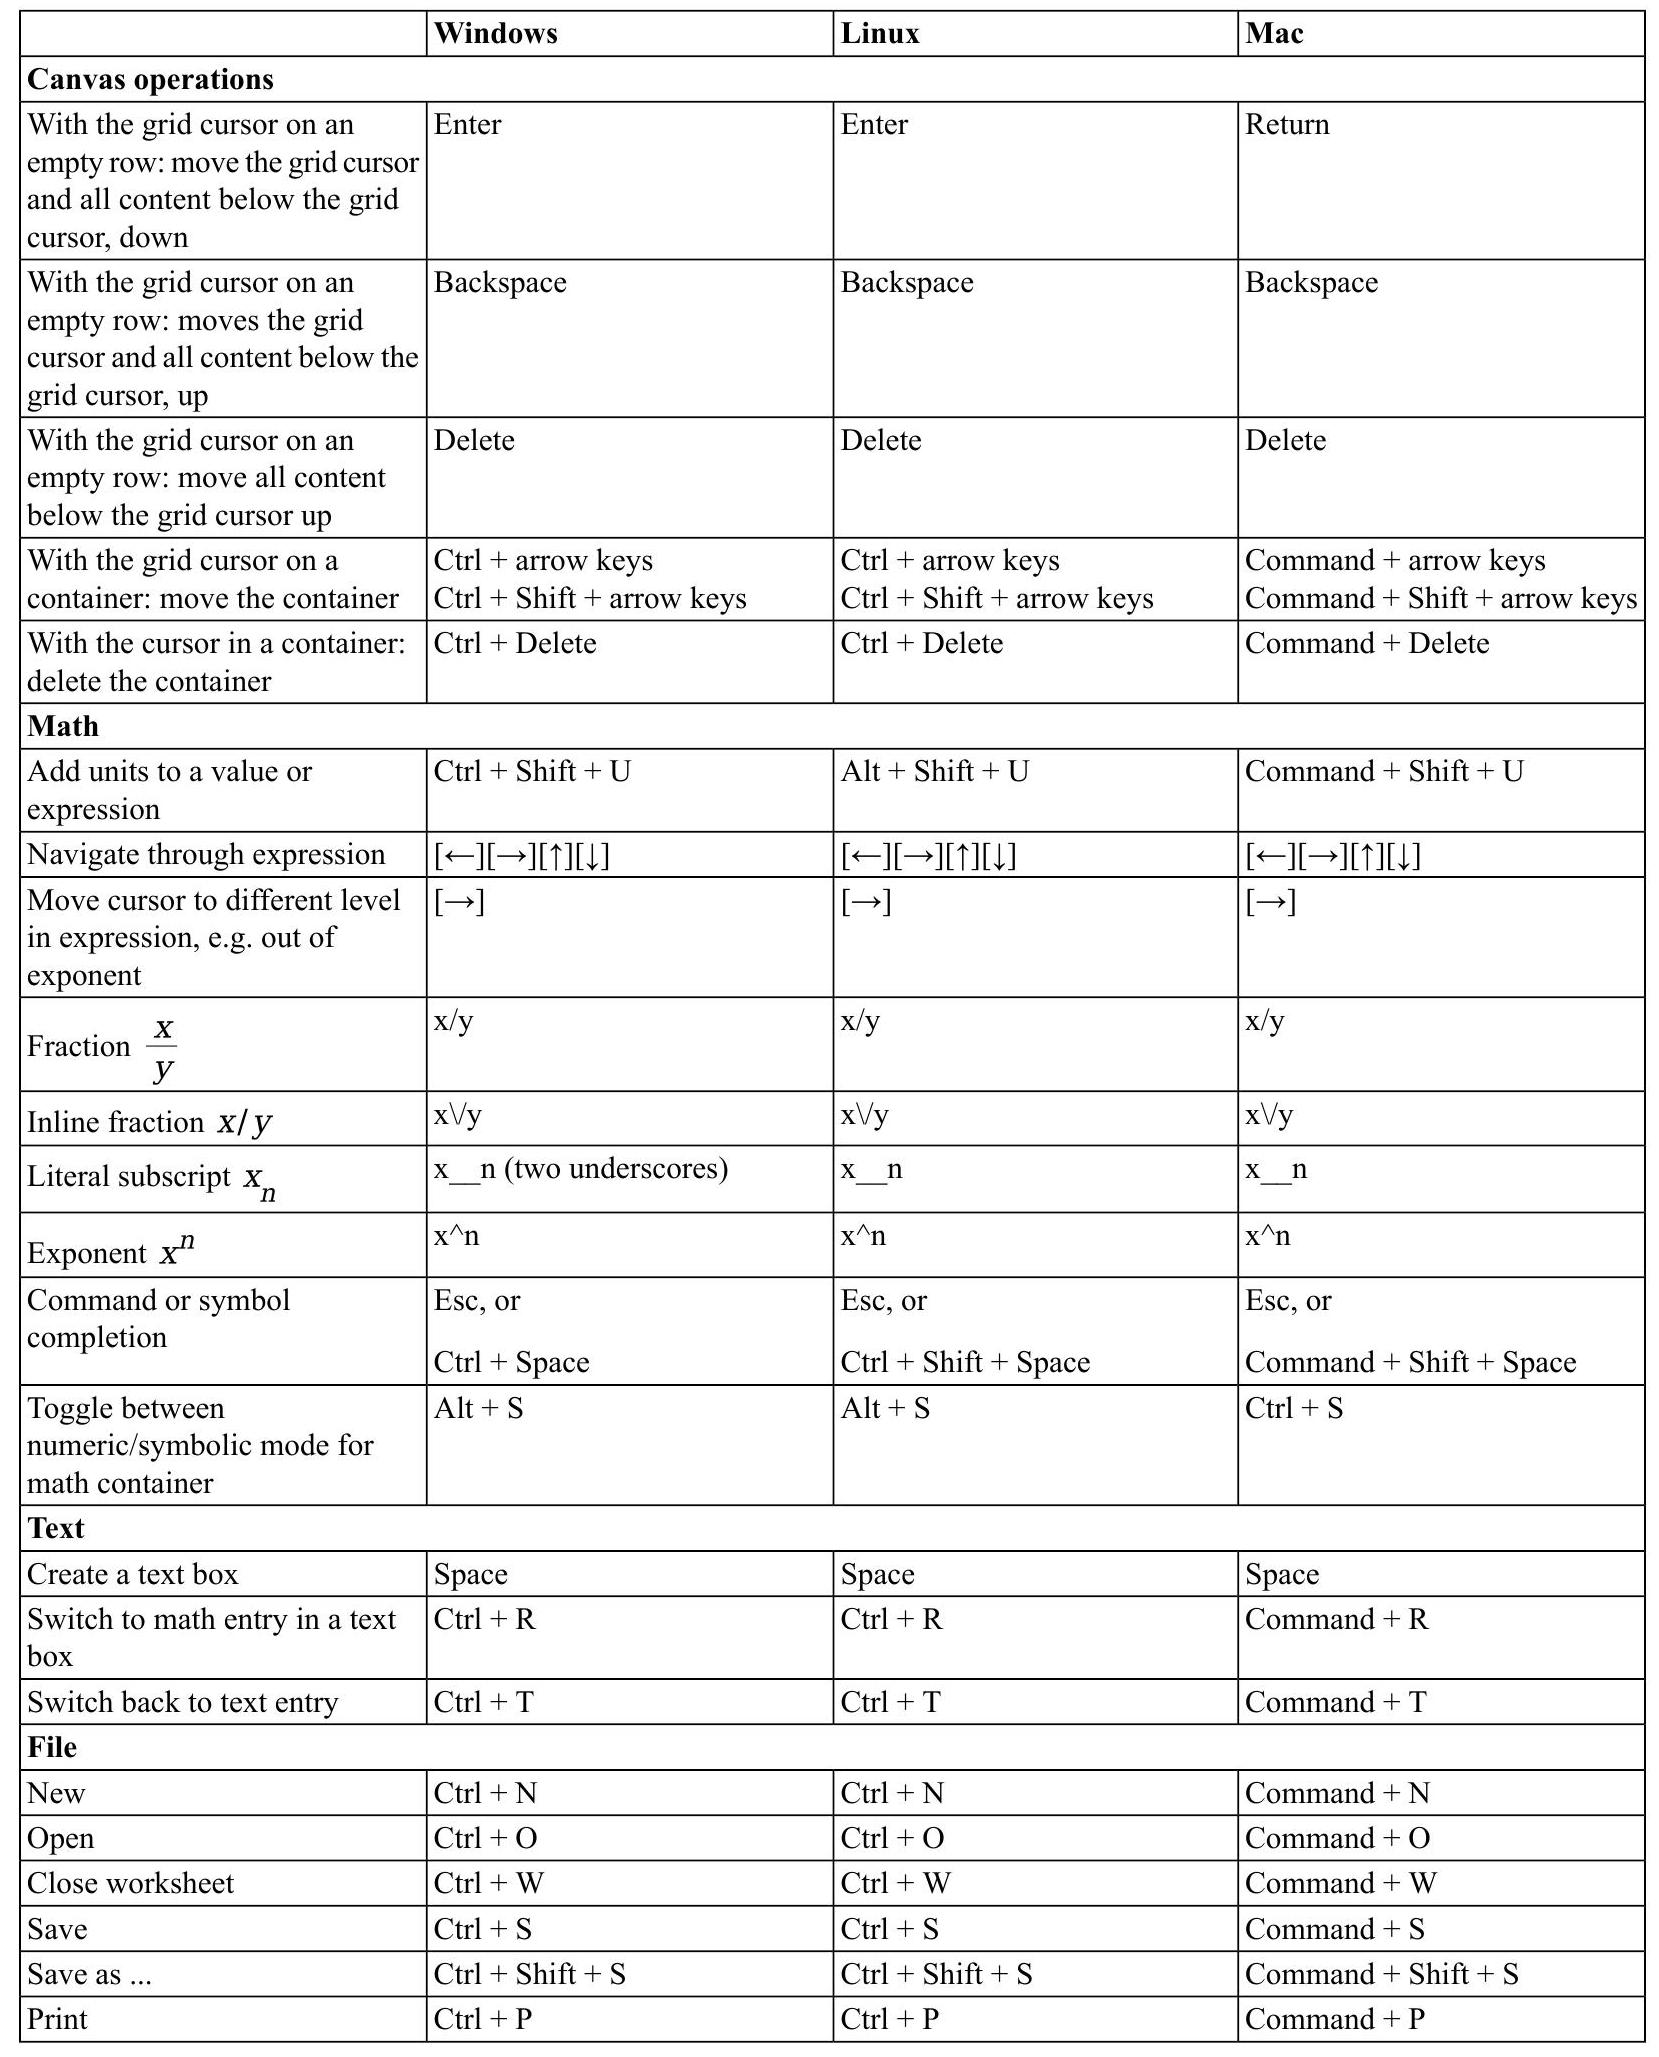
\includegraphics[max width=\textwidth]{2022_12_20_3e2ffe6ad124ec91ee5cg-40}
\end{center}

\begin{center}
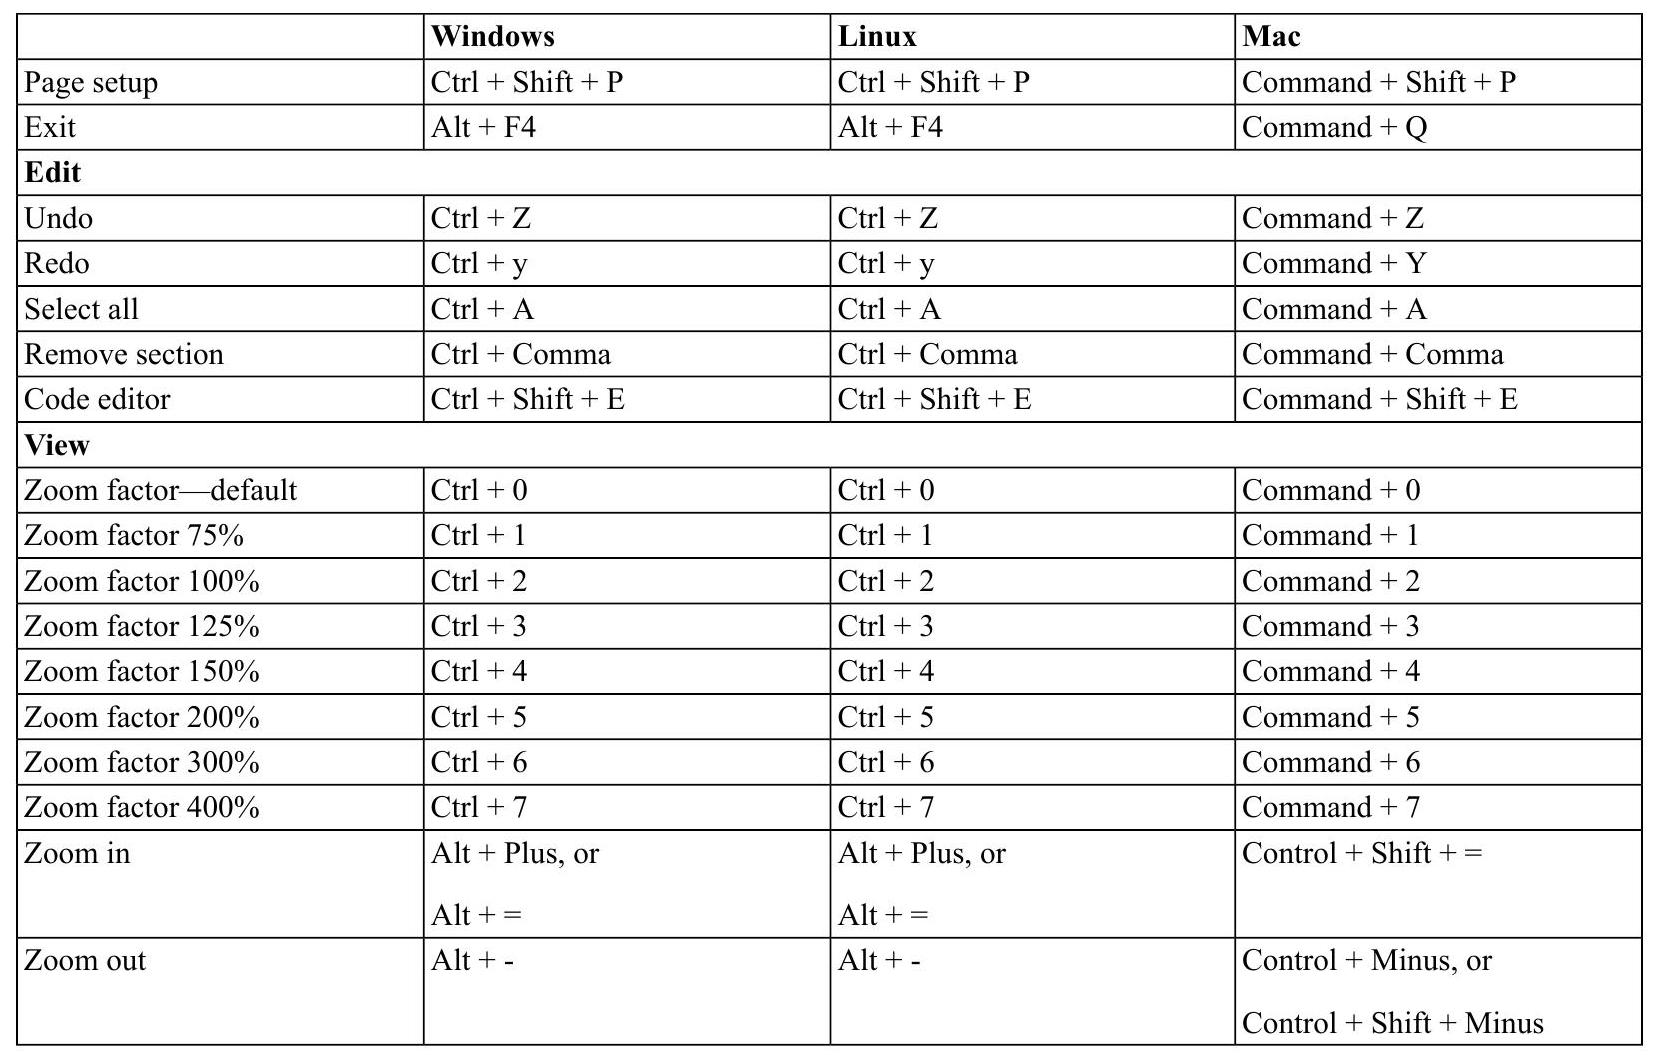
\includegraphics[max width=\textwidth]{2022_12_20_3e2ffe6ad124ec91ee5cg-41}
\end{center}

\section{Index}
\section{Symbols}
$:=, 11$

$=, 9$

